\documentclass[table]{beamer}
%[]中可以使用draft、handout、screen、transparency、trancompress、compress等参数

%指定beamer的模式与主题
\mode<presentation>
{
  \usetheme{Madrid}
%\usetheme{Boadilla}
%\usecolortheme{default}
%\usecolortheme{orchid}
%\usecolortheme{whale}
%\usefonttheme{professionalfonts}
}

%\usetheme{Madrid}
%这里还可以选择别的主题:Bergen, Boadilla, Madrid, AnnArbor, CambridgeUS, Pittsburgh, Rochester, Warsaw, ...
%有导航栏的Antibes, JuanLesPins, Montpellier, ...
%有内容的Berkeley, PaloAlto, Goettingen, Marburg, Hannover, ...
%有最小导航栏的Berlin, Ilmenau, Dresden, Darmstadt, Frankfurt, Singapore, Szeged, ...
%有章和节表单的Copenhagen, Luebeck, Malmoe, Warsaw, ...

%\usecolortheme{default}
%设置内部颜色主题(这些主题一般改变block里的颜色);这个主题一般选择动物来命名
%这里还可以选择别的颜色主题,如默认的和有特别目的的颜色主题default,structure,sidebartab,全颜色主题albatross,beetle,crane,dove,fly,seagull,wolverine,beaver

%\usecolortheme{orchid}
%设置外部颜色主题(这些主题一般改变title里的颜色);这个主题一般选择植物来命名
%这里还可以选择别的颜色主题,如默认的和有特别目的的颜色主题lily,orchid,rose

%\usecolortheme{whale}
%设置字体主题;这个主题一般选择海洋动物来命名
%这里还可以选择别的颜色主题,如默认的和有特别目的的颜色主题whale,seahorse,dolphin

%\usefonttheme{professionalfonts}
%类似的还可以定义structurebold,structuresmallcapsserif,professionalfonts

% 控制 beamer 的风格,可以根据自己的爱好修改
%\usepackage{beamerthemesplit} %使用 split 风格
%\usepackage{beamerthemeshadow} %使用 shadow 风格
%\usepackage[width=2cm,dark,tab]{beamerthemesidebar}

%插入音标
%\usepackage{tipa}
%\AtBeginDocument{
  %\renewcommand\textipa{\fontencoding{T3}\selectfont}
%}
%\AtBeginDocument{
  %\renewcommand\textipa[2][r]{{\fontfamily{cm#1}\tipaencoding #2}}
%}
%\renewenvironment{IPA}[1][r]
 %{\fontfamily{cm#1}\tipaencoding}
 %{}

% 设定英文字体
%\usepackage{fontspec}
% Fix bugs for fontspec in TeXLive2015
\ifdefined\suppressfontnotfounderror
  \expandafter\let\csname xetex_suppressfontnotfounderror:D\endcsname
    \suppressfontnotfounderror
\else
  \expandafter\let\csname xetex_suppressfontnotfounderror:D\endcsname
    \luatexsuppressfontnotfounderror
\fi
\usepackage[no-math]{fontspec}
\setmainfont{Times New Roman}
\setsansfont{Arial}
\setmonofont{Courier New}

% 设定中文字体
\usepackage[BoldFont,SlantFont,CJKchecksingle,CJKnumber]{xeCJK}
%\setCJKmainfont[BoldFont={Adobe Heiti Std},ItalicFont={Adobe Kaiti Std}]{Adobe Song Std}
\setCJKmainfont[BoldFont={Adobe Heiti Std},ItalicFont={Adobe Kaiti Std}]{WenQuanYi Micro Hei}
\setCJKsansfont{Adobe Heiti Std}
\setCJKmonofont{Adobe Fangsong Std}
\punctstyle{hangmobanjiao}

\defaultfontfeatures{Mapping=tex-text}
\usepackage{xunicode}
\usepackage{xltxtra}

\XeTeXlinebreaklocale "zh"
\XeTeXlinebreakskip = 0pt plus 1pt minus 0.1pt

\usepackage{setspace}
\usepackage{colortbl,xcolor}
\usepackage{hyperref}
%\hypersetup{xetex,bookmarksnumbered=true,bookmarksopen=true,pdfborder=1,breaklinks,colorlinks,linkcolor=blue,filecolor=black,urlcolor=cyan,citecolor=green}
\hypersetup{xetex,bookmarksnumbered=true,bookmarksopen=true,pdfborder=1,breaklinks,colorlinks,linkcolor=cyan,filecolor=black,urlcolor=blue,citecolor=green}

% 插入图片
\usepackage{graphicx}
\graphicspath{{figures/}}
% 图文混排
%\usepackage{picins}
\usepackage{floatflt}

% 可能用到的包
\usepackage{amsmath,amssymb}
%插入多媒体
%\usepackage{media9}
%\usepackage{movie15}
\usepackage{multimedia}
\usepackage{multicol}
\usepackage{multirow}

% 定义一些自选的模板,包括背景、图标、导航条和页脚等,修改要慎重
% 设置背景渐变由10%的红变成10%的结构颜色
%\beamertemplateshadingbackground{red!10}{structure!10}
%\beamertemplatesolidbackgroundcolor{white!90!blue}
% 使所有隐藏的文本完全透明、动态,而且动态的范围很小
\beamertemplatetransparentcovereddynamic
% 使itemize环境中变成小球,这是一种视觉效果
\beamertemplateballitem
% 为所有已编号的部分设置一个章节目录,并且编号显示成小球
\beamertemplatenumberedballsectiontoc
% 将每一页的要素的要素名设成加粗字体
\beamertemplateboldpartpage

% item逐步显示时,使已经出现的item、正在显示的item、将要出现的item呈现不同颜色
\def\hilite<#1>{
 \temporal<#1>{\color{gray}}{\color{blue}}
    {\color{blue!25}}
}

\renewcommand{\today}{\number\year 年 \number\month 月 \number\day 日}

%五角星
\usepackage{MnSymbol}

%去除图表标题中的figure等
\usepackage{caption}
\captionsetup{labelformat=empty,labelsep=none}

\usepackage{tabu}
\usepackage{multirow}
%表格自动换行
\usepackage{tabularx} 

% 千分号
%\usepackage{textcomp}

%罗马数字
\makeatletter
\newcommand{\rmnum}[1]{\romannumeral #1}
\newcommand{\Rmnum}[1]{\expandafter\@slowromancap\romannumeral #1@}
\makeatother

%分栏
\usepackage{multicol}

%\usepackage{enumitem}
%\usepackage{enumerate}

%键盘
\usepackage{keystroke}

%插入源代码
\usepackage{listings}
\lstset{
  language=perl,                  % 程序语言名称:TeX, Perl, R, sh, bash, Awk
  basicstyle=\normalsize\tt,      %\tt指monospace字体族,程序源代码使用此族字体表示更加美观
  numbers=left,                   % 行号位置(左侧)
  numberstyle=\small,             % 行号字体的字号
  stepnumber=1,                   % 行号的显示步长
  numbersep=5pt,                  % 行号与代码间距
  backgroundcolor=\color{white},  % 背景色;需要 \usepackage{color}
  showspaces=false,               % 不显示空格
  showstringspaces=false,         % 不显示代码字符串中的空格标记
  showtabs=false,                 % 不显示 TAB
  tabsize=4, 
  frame=shadowbox,                % 把代码用带有阴影的框圈起来
  captionpos=b,                   % 标题位置
  breaklines=true,                % 对过长的代码自动断行
  breakatwhitespace=false,        % 断行只在空格处
  extendedchars=false,            % 解决代码跨页时,章节标题,页眉等汉字不显示的问题
  %escapeinside={\%*}{*},         % 跳脱字符,添加注释,暂时离开 listings 
  %escapeinside=``,
  commentstyle=\color{red!50!green!50!blue!50}\tt,  %浅灰色的注释
  rulesepcolor=\color{red!20!green!20!blue!20},     %代码块边框为淡青色
  keywordstyle=\color{blue!70}\bfseries\tt,         %代码关键字的颜色为蓝色,粗体
  identifierstyle=\tt,
  stringstyle=\tt,                % 代码字符串的特殊格式
  keepspaces=true,
  breakindent=1em,
  %breakindent=22pt,
  %breakindent=4em,
  breakautoindent=true,
  flexiblecolumns=true,
  aboveskip=1em,                  %代码块边框
  xleftmargin=2em,
  xrightmargin=2em
}

%\setbeamercolor{alerted text}{fg=magenta}
\setbeamercolor{bgcolor}{fg=yellow,bg=cyan}
%\setbeamercolor{itemize/enumerate body}{fg=green}

\begin{document}

%\includeonlyframes{current}

\logo{
\includegraphics[height=0.08\textwidth]{tijmu.png}}

% 在每个Section前都会加入的Frame
\AtBeginSection[]
{
  \begin{frame}<beamer>
    %\frametitle{Outline}
    \frametitle{教学提纲}
    \setcounter{tocdepth}{3}
    \begin{multicols}{2}
      \tableofcontents[currentsection,currentsubsection]
      %\tableofcontents[currentsection]
    \end{multicols}
  \end{frame}
}
% 在每个Subsection前都会加入的Frame
\AtBeginSubsection[]
{
  \begin{frame}<beamer>
%%\begin{frame}<handout:0>
%% handout:0 表示只在手稿中出现
    \frametitle{教学提纲}
    \setcounter{tocdepth}{3}
    \begin{multicols}{2}
    \tableofcontents[currentsection,currentsubsection]
    \end{multicols}
%% 显示在目录中加亮的当前章节
  \end{frame}
}

% 为当前幻灯片设置背景
%{
%\usebackgroundtemplate{
%\vbox to \paperheight{\vfil\hbox to
%\paperwidth{\hfil
\includegraphics[width=2in]{tijmu_charcoal.png}\hfil}\vfil}
%}
\begin{frame}[plain]
  \begin{center}
    {\Huge 分子生物计算\\}
    {\huge \textit{(Perl语言编程)}\\}
    \vspace{1cm}
    {\LARGE 天津医科大学\\}
    %\vspace{0.2cm}
    {\LARGE 生物医学工程与技术学院\\}
    \vspace{1cm}
    {\large 2016-2017学年上学期(秋)\\ 2014级生信班}
  \end{center}
\end{frame}
%}



%\includeonlyframes{current}

\title[绪论]{第一章\quad 绪论}
\author[Yixf]{伊现富(Yi Xianfu)}
\institute[TIJMU]{天津医科大学(TIJMU)\\ 生物医学工程与技术学院}
\date{2015年9月}

\begin{frame}
  \titlepage
\end{frame}

\begin{frame}[plain,label=current]
  \frametitle{教学提纲}
  \setcounter{tocdepth}{3}
  \begin{multicols}{2}
    \tableofcontents
  \end{multicols}
\end{frame}


\section{课程安排}
\begin{frame}
  \frametitle{课程安排 | 授课教材}
  \begin{figure}
    \centering
    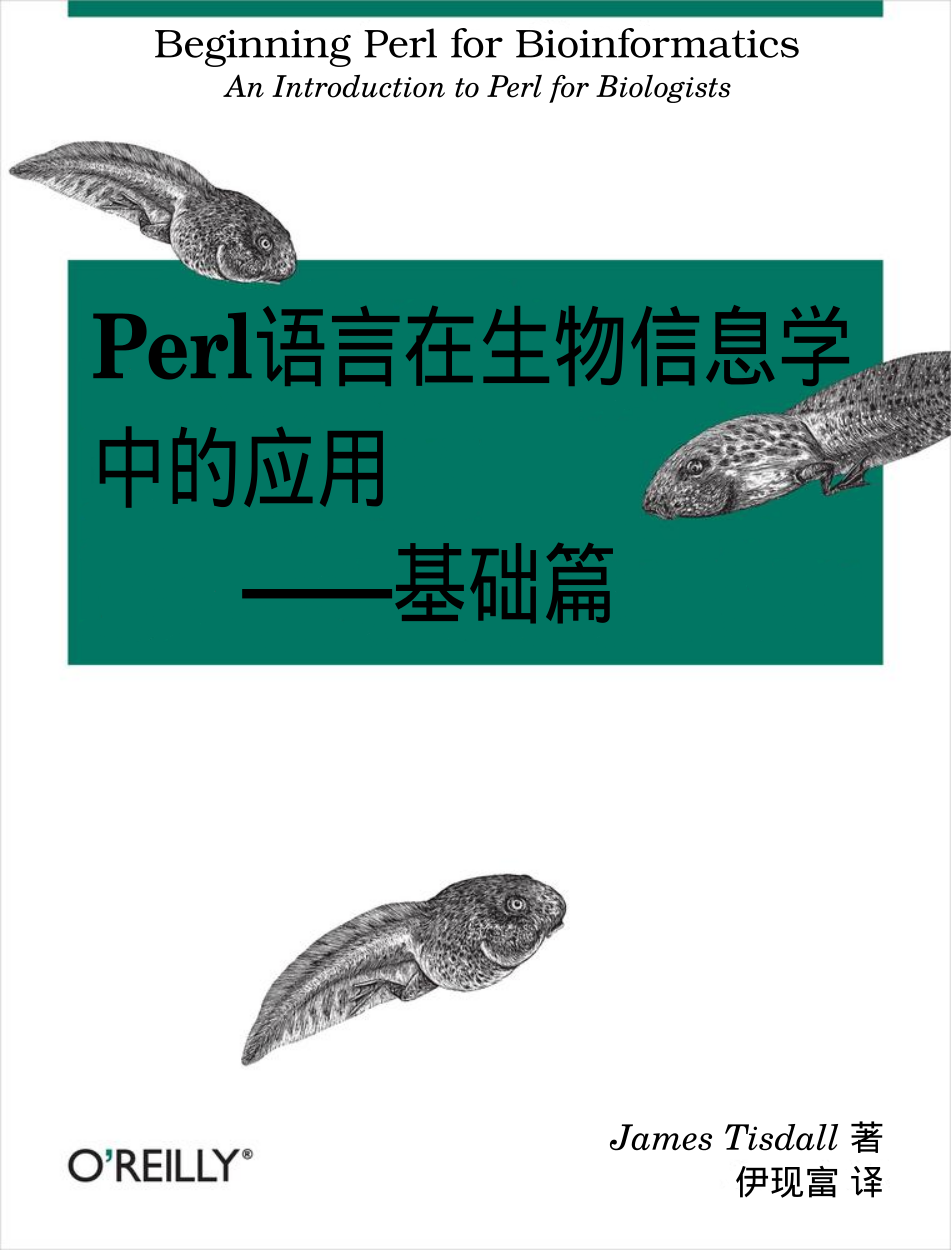
\includegraphics[width=6cm]{c1.intro.textbook.png}
  \end{figure}
\end{frame}

\begin{frame}
  \frametitle{课程安排 | 理论课}
  \begin{center}
  \alert{后9周,每周三,下午四节(13:30-17:30),西楼610}\\
  \vspace{0.2cm}
  \end{center}
  \begin{block}{授课内容}
    \begin{itemize}
      \item 教材内容:第一章……~第十章
      \item 补充知识:Markdown, Git, ...
    \end{itemize}
  \end{block}
\end{frame}

\begin{frame}
  \frametitle{课程安排 | 理论课 | 自主学习}
  \begin{itemize}
    \item 上课期间以小组形式编写程序
    \item 任务主题不限(生信方面的最好)
    \item 理论课的最后一/两次课(2~4学时)进行报告
    \item 小组成员人人都要参与
    \item 既参与编程又进行报告者加分
    \item 作为平时成绩的一大部分
  \end{itemize}
\end{frame}

\begin{frame}
  \frametitle{课程安排 | 理论课 | 自主学习 | 实例}
  \begin{block}{目的}
    按照用户的需求生成随机密码。
  \end{block}
  \pause
  \begin{block}{需求}
    \begin{itemize}
      \item 指定生成密码的元素(默认:混合使用数字、大小写字母、符号)
      \item 指定生成密码的长度(默认:12个字符)
      \item 指定生成密码的个数(默认:1个)
      \item 指定密码中元素的比例/字符数(默认:无比例/字符数要求)
      \item 指定需要排除的元素(比如:0和O,1和l;默认:无)
      \item 挖掘更多人性化需求……
    \end{itemize}
  \end{block}
  \pause
  \begin{block}{代码仓库}
    \begin{itemize}
      \item \href{https://github.com/Yixf-Education/project_Perl}{Yixf-Education/project\_Perl}
    \end{itemize}
  \end{block}
\end{frame}

\begin{frame}
  \frametitle{课程安排 | 实验课}
  \begin{center}
  \alert{后9周,每周四,上午后两节(10:10-12:00),教一楼304}\\
  \vspace{0.2cm}
  \end{center}
  \begin{block}{实验内容}
    \begin{itemize}
      \item 紧跟理论课进度
      \item 教材上的程序/实例
    \end{itemize}
  \end{block}
\end{frame}

\begin{frame}
  \frametitle{课程安排 | 考核方式}
  \begin{enumerate}
    \item 理论课:60\%
      \begin{enumerate}
        \item 平时表现:10\%
        \item 闭卷考试:50\%
      \end{enumerate}
    \item 实验课:40\%
      \begin{enumerate}
        \item 平时表现:20\%
        \item 实验报告:20\%
      \end{enumerate}
  \end{enumerate}
\end{frame}



\section{生物信息学}
\begin{frame}
  \frametitle{生物信息学(bioinformatics)}
  \begin{quotation}
    ``If you can't do bioinformatics, you can't do biology."
    \begin{flushright}
    Lincoln Stein\\
    (Biologist and former CSHL Professor)
  \end{flushright}
  \end{quotation}
  \vspace{-1em}
  \begin{figure}
    \centering
    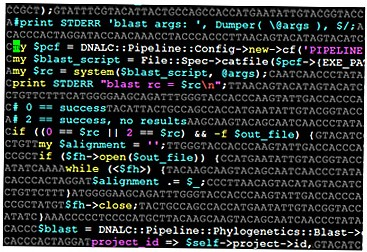
\includegraphics[width=8cm]{c1.intro.code.jpg}
  \end{figure}
\end{frame}

\begin{frame}
  \frametitle{生物信息学 | 维基百科}
  生物信息学(bioinformatics)利用应用数学、信息学、统计学和计算机科学的方法研究生物学的问题。目前的生物信息学基本上只是分子生物学与信息技术(尤其是互联网技术)的结合体。\\
  \vspace{1em}
  生物信息学的研究材料和结果就是各种各样的生物学数据,其研究工具是计算机,研究方法包括对生物学数据的搜索(收集和筛选)、处理(编辑、整理、管理和显示)及利用(计算、模拟)。\\
  \vspace{1em}
  目前主要的研究方向有:序列比对、基因识别、基因重组、蛋白质结构预测、基因表达、蛋白质反应的预测,以及建立进化模型。
\end{frame}

\begin{frame}
  \frametitle{生物信息学 | 维基百科(续)}
  生物学技术往往生成大量的嘈杂数据。与数据挖掘类似,生物信息学利用数学工具从大量数据中提取有用的生物学信息。生物信息学所要处理的典型问题包括:重新组装在霰弹枪测序法测序过程中被打散的DNA序列,从蛋白质的氨基酸序列预测蛋白质结构,利用mRNA微阵列或质谱仪的数据检验基因调控的假说。\\
  \vspace{1em}
  某些人将计算生物学作为生物信息学的同义词处理;但是另外一些人认为计算生物学和生物信息学应当被当作不同的条目处理,因为生物信息学更侧重于生物学领域中计算方法的使用和发展,而计算生物学强调应用信息学技术对生物学领域中的假说进行检验,并尝试发展新的理论。
\end{frame}

\begin{frame}
  \frametitle{生物信息学 | 维基百科(续)}
  生物信息学可以定义为对分子生物学中两类信息流的研究:\\
  \vspace{1em}
  第一类信息流源于分子生物学的中心法则:DNA序列被转录为mRNA序列,后者被翻译为蛋白质序列。蛋白质序列继而折叠为具有功能的三维结构。按照达尔文演化理论,这些功能被生物体的环境所选择,从而驱动群体中DNA序列的进化。因此,第一类的生物信息学应用关注于中心法则中任一阶段的信息传递,包括DNA序列中基因的组织与控制、确定DNA中的转录单位、从序列预测蛋白质结构以及分子功能分析。\\
  \vspace{1em}
  第二类信息流是基于科学方法:提出关于生物学活动的假设,设计实验以验证这些假设,评估结果与假设的相容性,然后根据实验数据对原假设作扩展或修正。第二类的生物信息学应用关注于这一流程中的信息传递,包括产生假设、设计实验、通过数据库将实验结果组织起来、检验数据与模型的相容性以及修正假设的各个系统。
\end{frame}

\begin{frame}
  \frametitle{生物信息学 | 是什么? | 学科角度}
  \begin{figure}
    \centering
    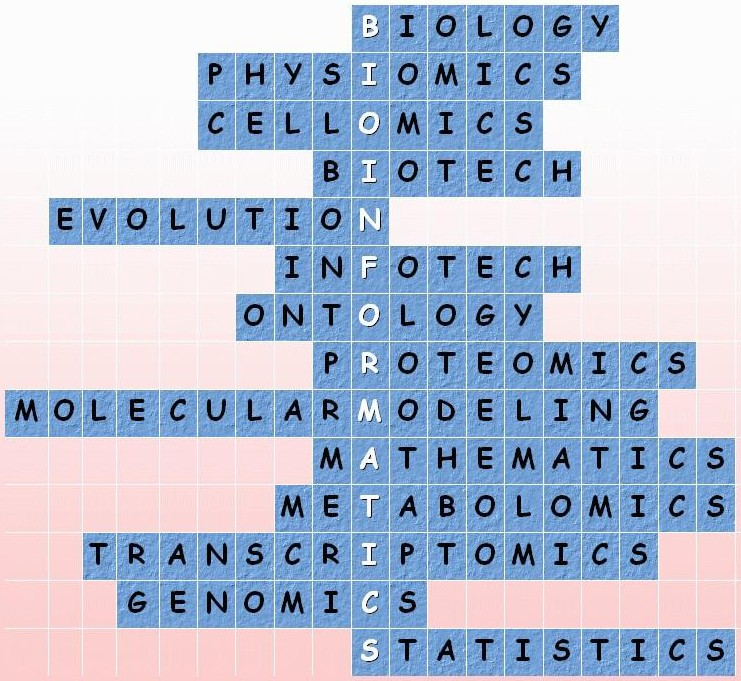
\includegraphics[width=10.5cm,height=7.5cm]{c1.intro.bioinfo.what.01.jpg}
  \end{figure}
\end{frame}

\begin{frame}
  \frametitle{生物信息学 | 是什么? | 学科角度}
  \begin{figure}
    \centering
    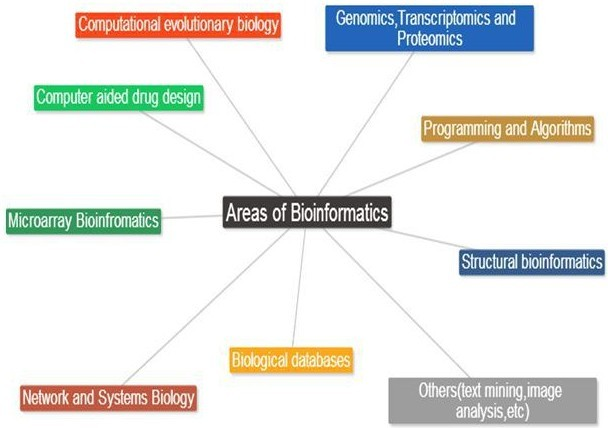
\includegraphics[width=10cm]{c1.intro.bioinfo.what.02.jpg}
  \end{figure}
\end{frame}

\begin{frame}
  \frametitle{生物信息学 | 是什么? | \alert{学科角度}}
  \begin{figure}
    \centering
    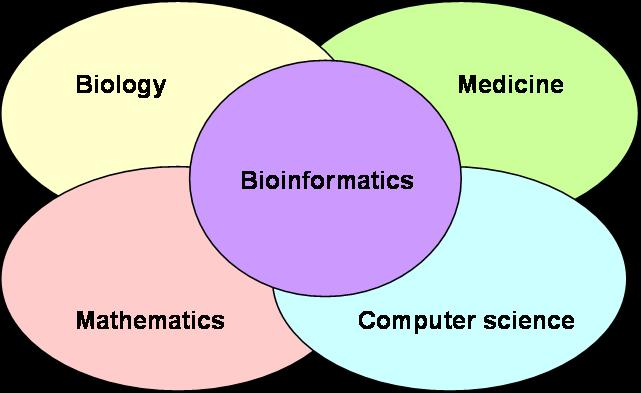
\includegraphics[width=10cm]{c1.intro.bioinfo.what.03.jpg}
  \end{figure}
\end{frame}

\begin{frame}
  \frametitle{生物信息学 | 是什么? | \alert{技术角度}}
  \begin{figure}
    \centering
    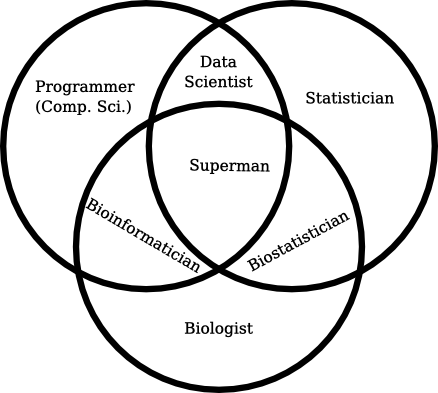
\includegraphics[width=8.5cm]{c1.intro.bioinfo.what.04.png}
  \end{figure}
\end{frame}

\begin{frame}
  \frametitle{生物信息学 | \alert{做什么?}}
  \begin{figure}
    \centering
    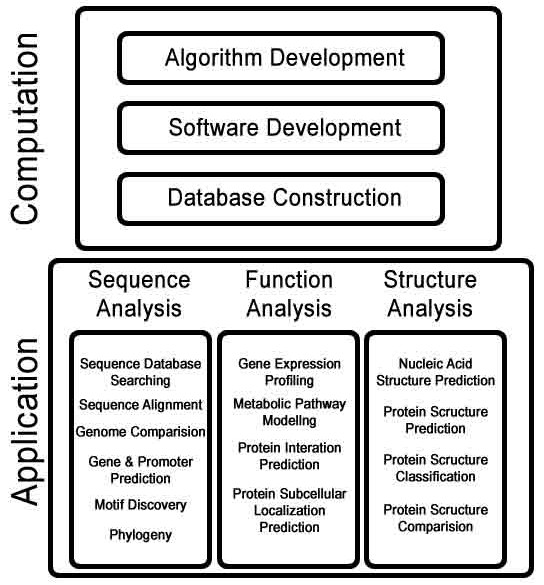
\includegraphics[width=7cm]{c1.intro.bioinfo.do.jpg}
  \end{figure}
\end{frame}

\begin{frame}
  \frametitle{生物信息学 | 资源(数据库与工具)}
  \begin{figure}
    \centering
    
\includegraphics[width=10.5cm]{c1.intro.bioinfo.resource.png}
  \end{figure}
\end{frame}

\begin{frame}
  \frametitle{生物信息学 | 资源(技术与工具)}
  \begin{figure}
    \centering
    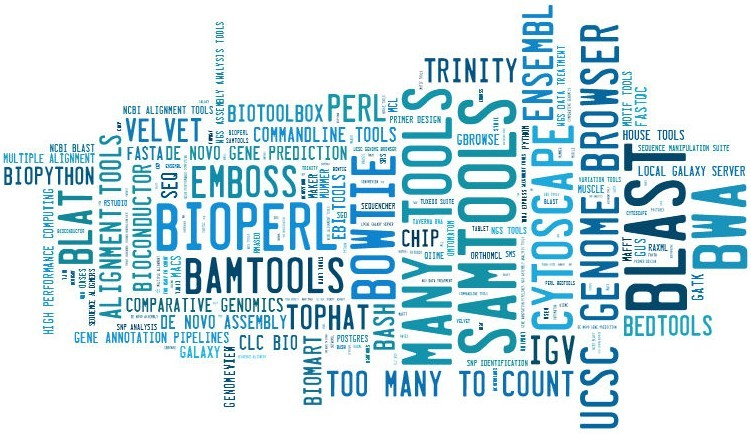
\includegraphics[width=11cm]{c1.intro.bioinfo.tool.01.jpg}
  \end{figure}
\end{frame}

\begin{frame}
  \frametitle{生物信息学 | 主题词}
  \begin{figure}
    \centering
    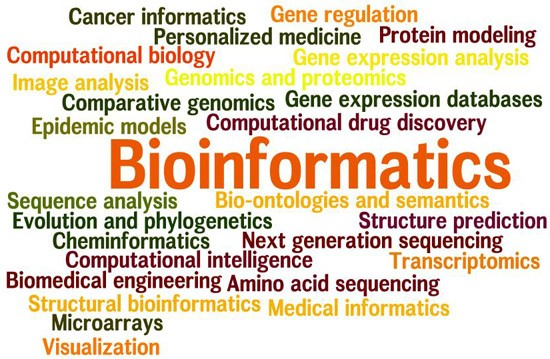
\includegraphics[width=10.5cm]{c1.intro.bioinfo.topic.01.jpg}
  \end{figure}
\end{frame}

\begin{frame}
  \frametitle{生物信息学 | 主题词}
  \begin{figure}
    \centering
    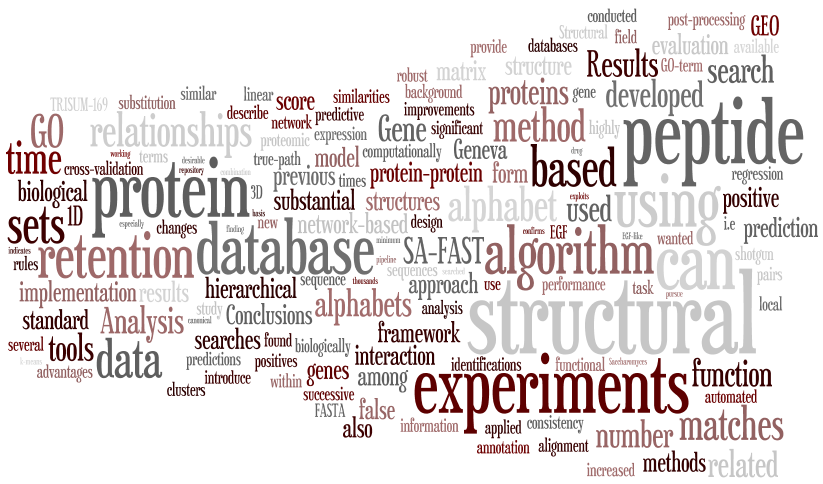
\includegraphics[width=10.5cm]{c1.intro.bioinfo.topic.02.png}
  \end{figure}
\end{frame}

\section{生物学}
\begin{frame}
  \frametitle{生物学 | 历史}
  \begin{figure}
    \centering
    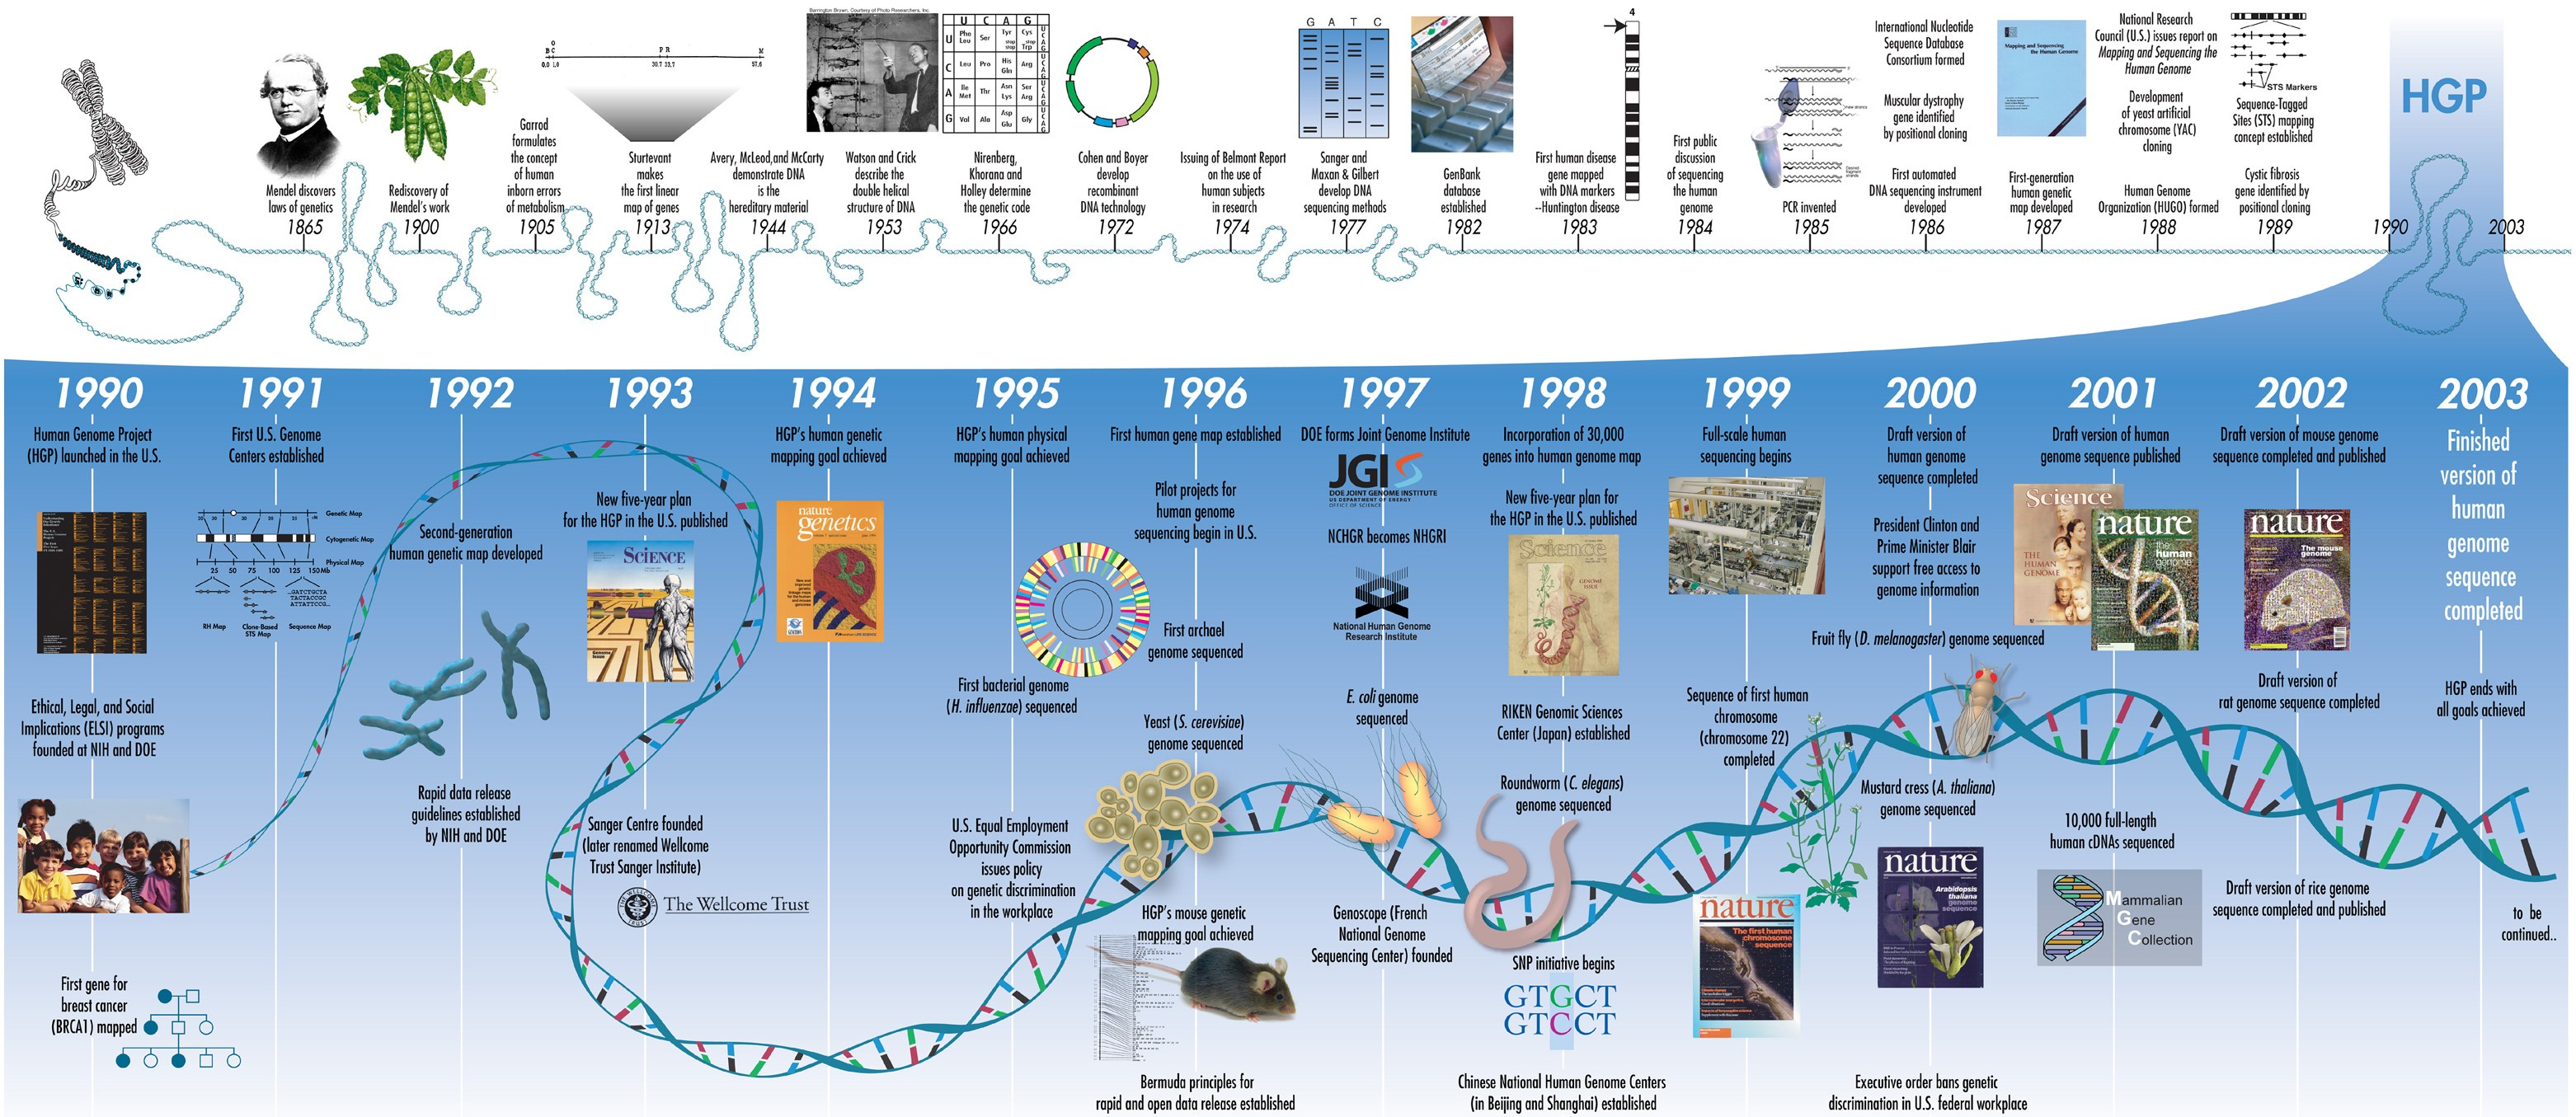
\includegraphics[width=12cm]{c1.intro.biology.history.01.jpg}
  \end{figure}
\end{frame}

\begin{frame}
  \frametitle{生物学 | 中心法则(central dogma)}
  \begin{figure}
    \centering
    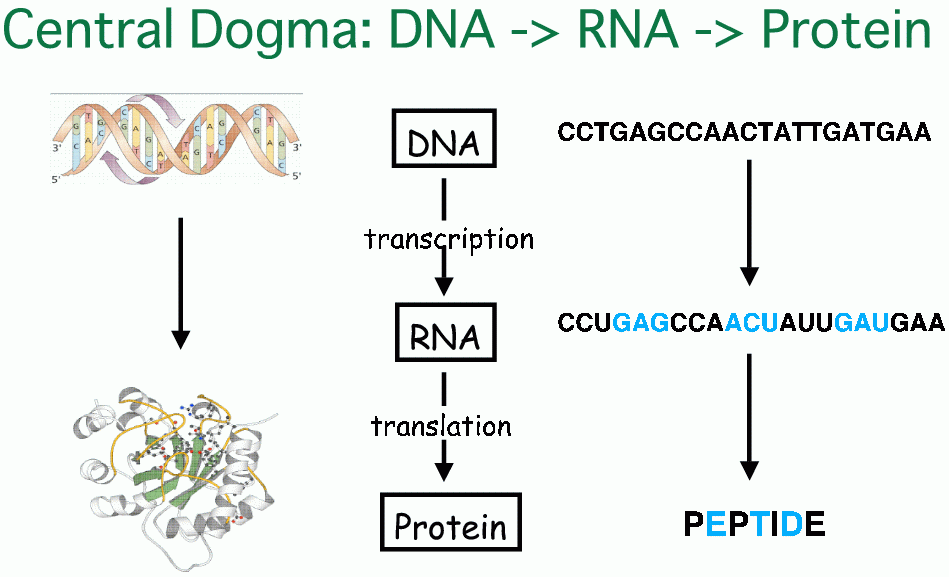
\includegraphics[width=10.5cm]{c1.intro.dogma.01.png}
  \end{figure}
\end{frame}

\begin{frame}
  \frametitle{生物学 | \alert{DNA}}
  \begin{figure}
    \centering
    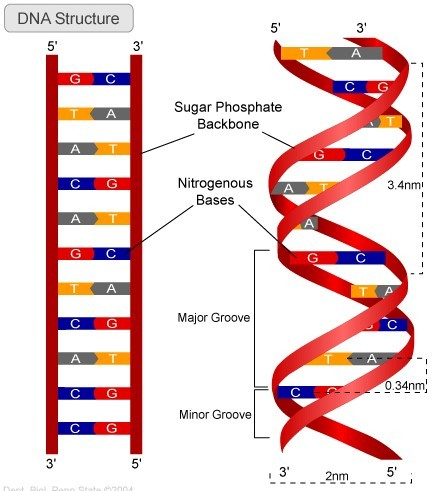
\includegraphics[width=7cm]{c1.intro.dna.01.jpg}
  \end{figure}
\end{frame}

\begin{frame}
  \frametitle{生物学 | \alert{RNA}}
  \begin{figure}
    \centering
    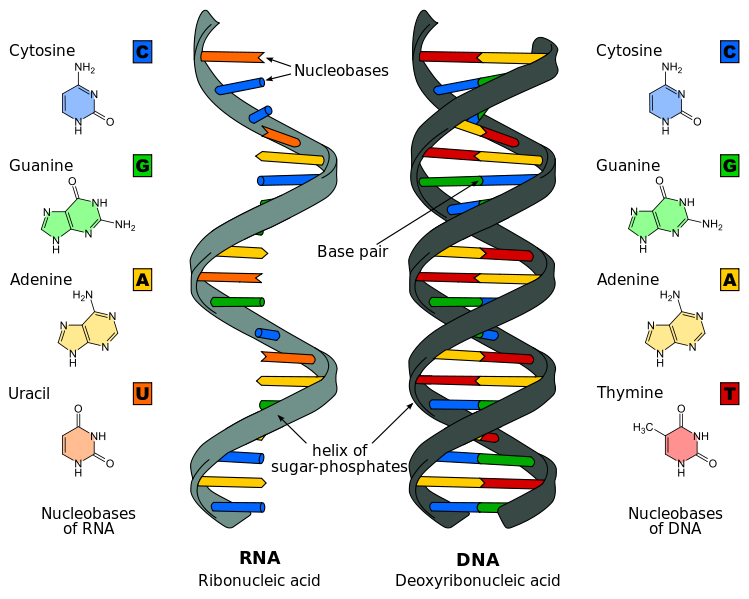
\includegraphics[width=9.5cm]{c1.intro.rna.01.png}
  \end{figure}
\end{frame}

\begin{frame}
  \frametitle{生物学 | 蛋白质 | \alert{氨基酸}}
  \begin{figure}
    \centering
    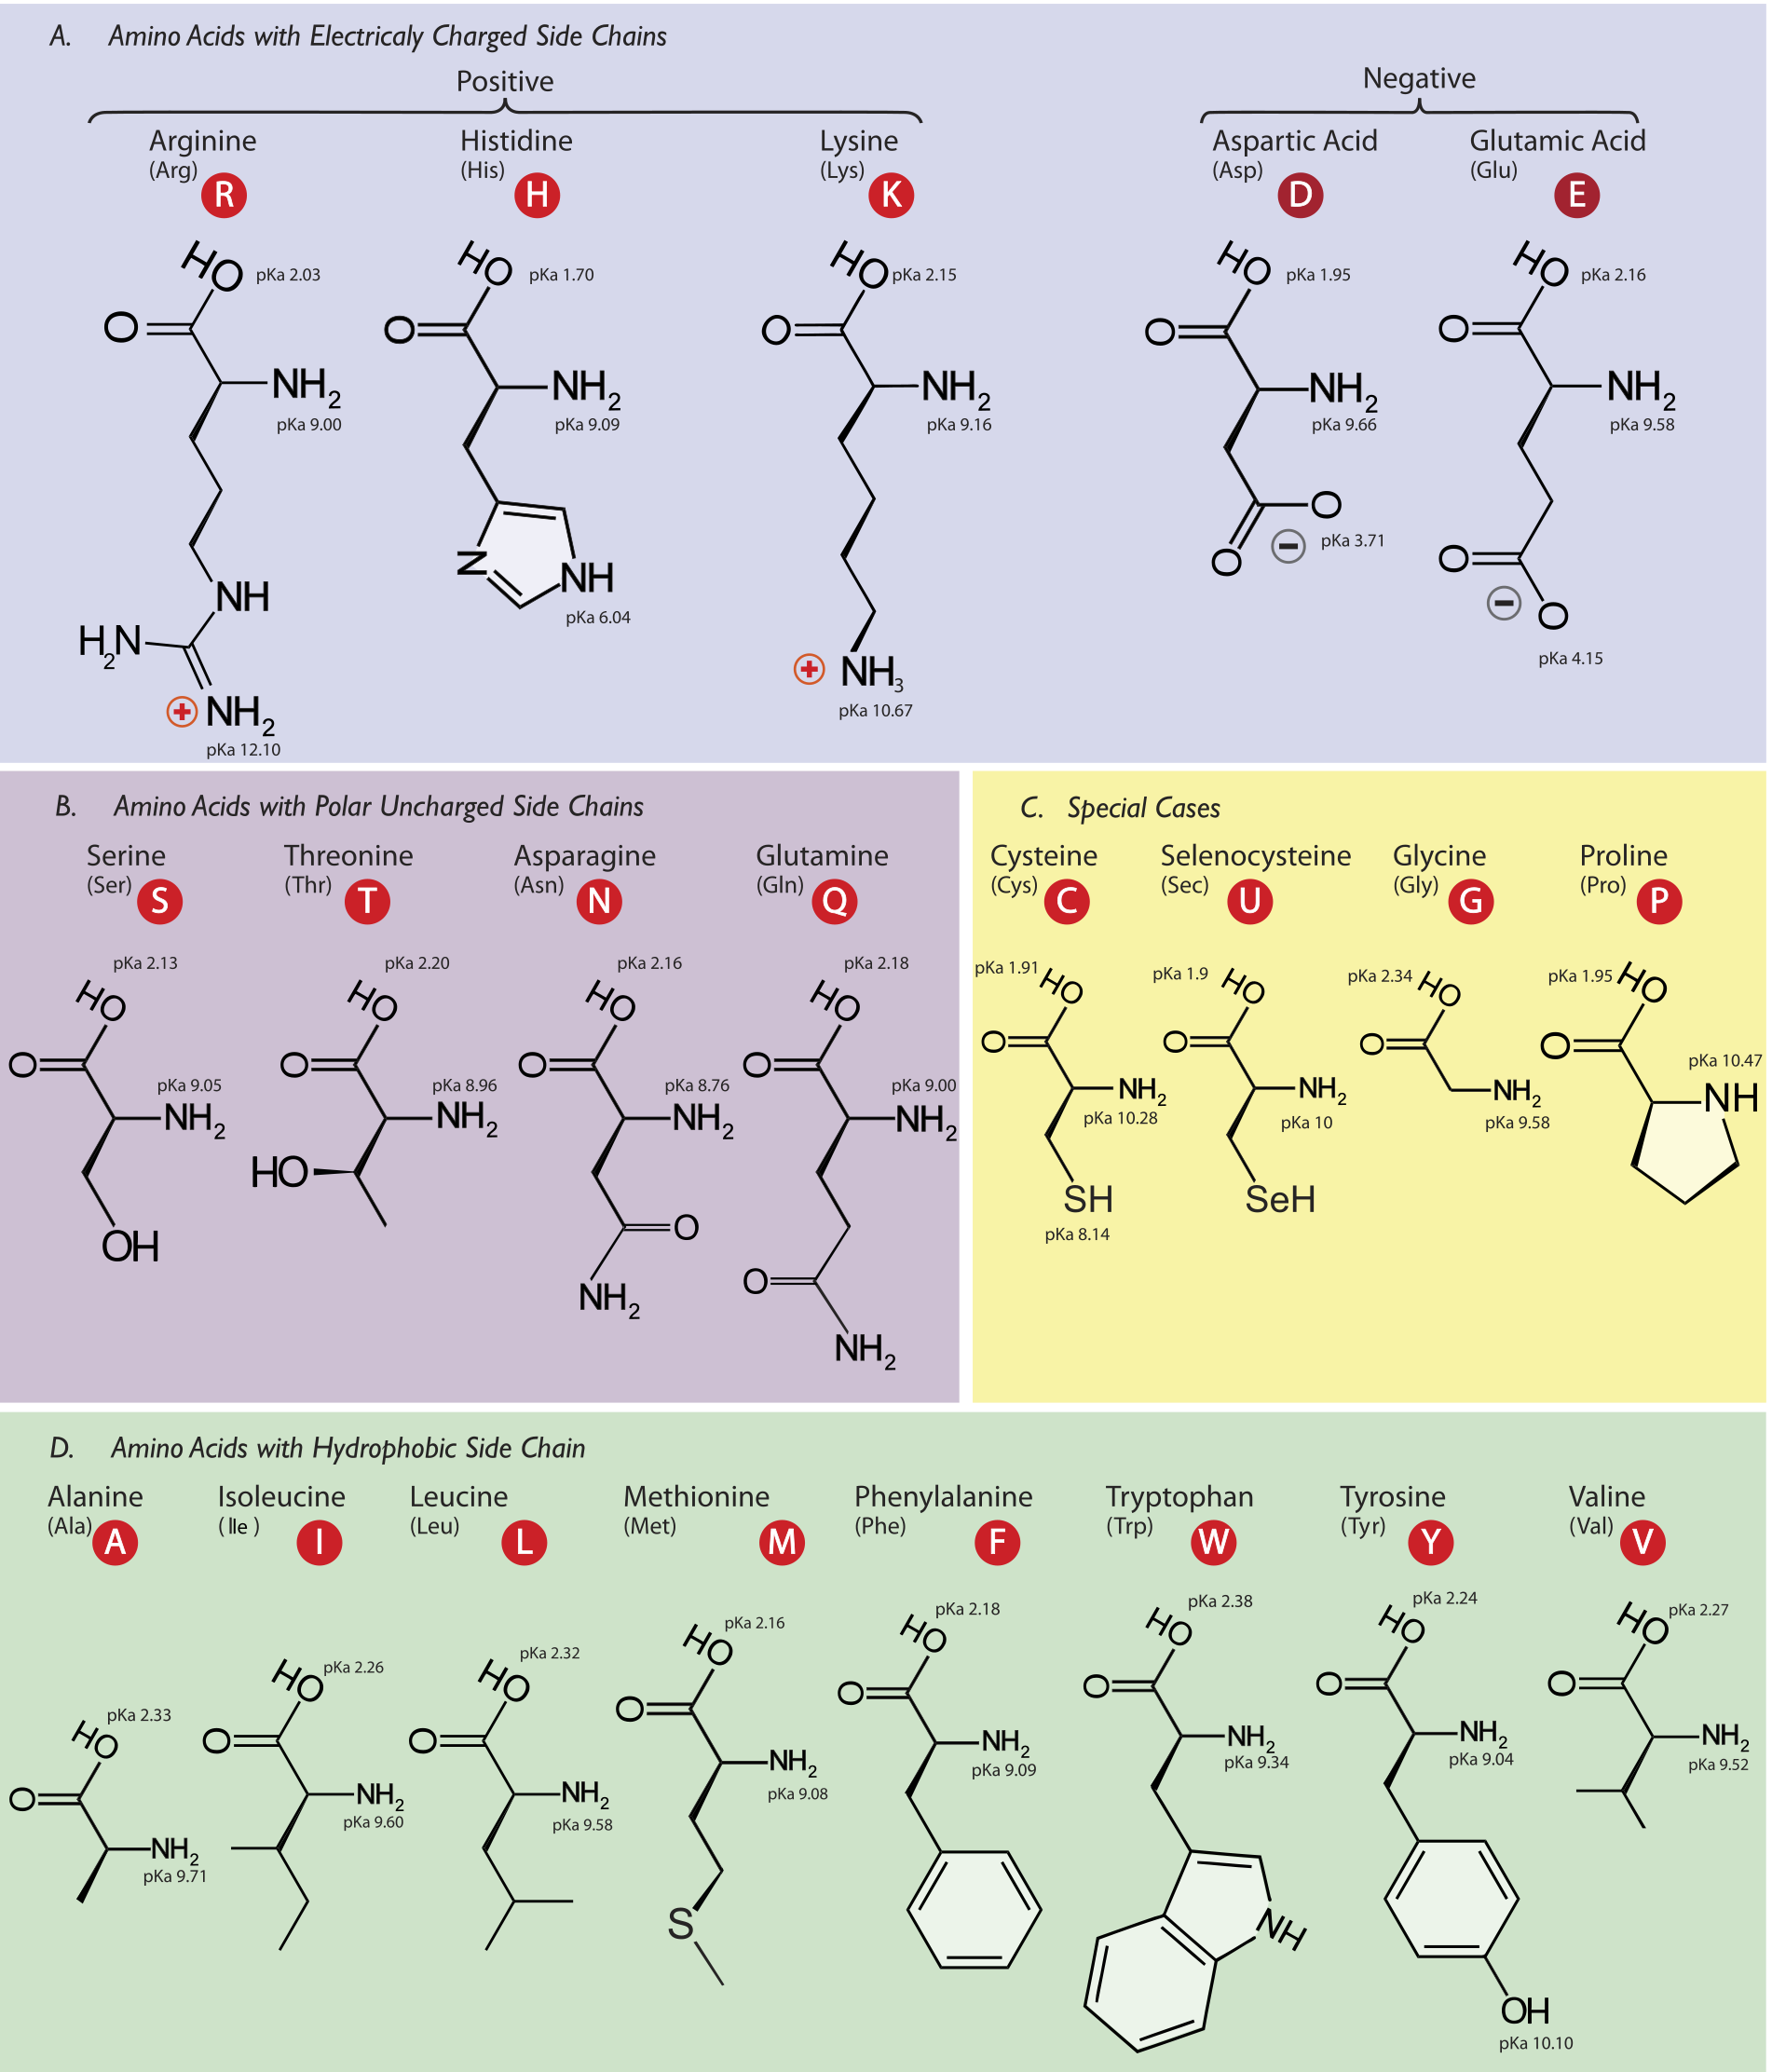
\includegraphics[width=9.5cm,height=7.5cm]{c1.intro.aa.01.png}
  \end{figure}
\end{frame}

\begin{frame}
  \frametitle{生物学 | 蛋白质 | 氨基酸 | 助记口诀}
  \begin{block}{必需氨基酸}
  甲携来一本亮色书(甲硫氨酸、缬氨酸、赖氨酸、异亮氨酸、苯丙氨酸、亮氨酸、色氨酸、苏氨酸)
\end{block}
\pause
\begin{block}{20种氨基酸}
  苏缬亮异亮,苯丙属芳香。\\
  还有色赖蛋,缺一人遭殃。\\
  (以上是必需氨基酸)\\
  丙组丝甘半,天谷建酸胺。\\
  精酪加一脯,20氨基酸。\\
  (以上是非必需氨基酸)
\end{block}
\end{frame}

\begin{frame}
  \frametitle{生物学 | 蛋白质 | 多肽}
  \begin{figure}
    \centering
    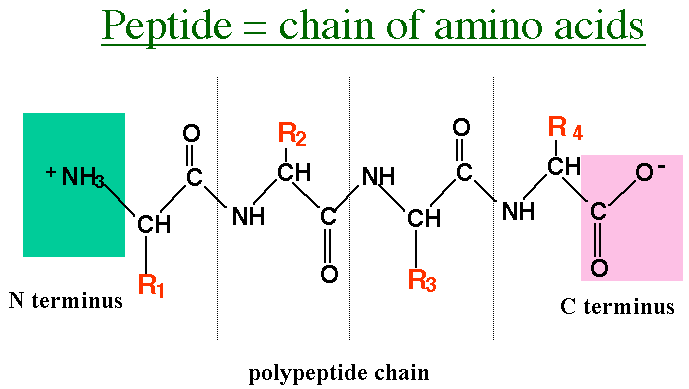
\includegraphics[width=8cm,height=3cm]{c1.intro.peptide.01.png}\\
    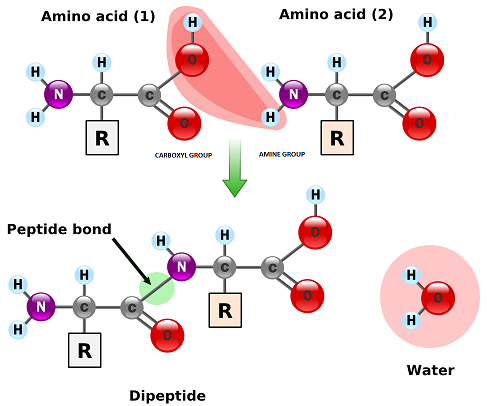
\includegraphics[width=7cm,height=4.8cm]{c1.intro.peptide.02.png}
  \end{figure}
\end{frame}

\begin{frame}
  \frametitle{生物学 | 蛋白质 | 结构}
  \begin{figure}
    \centering
    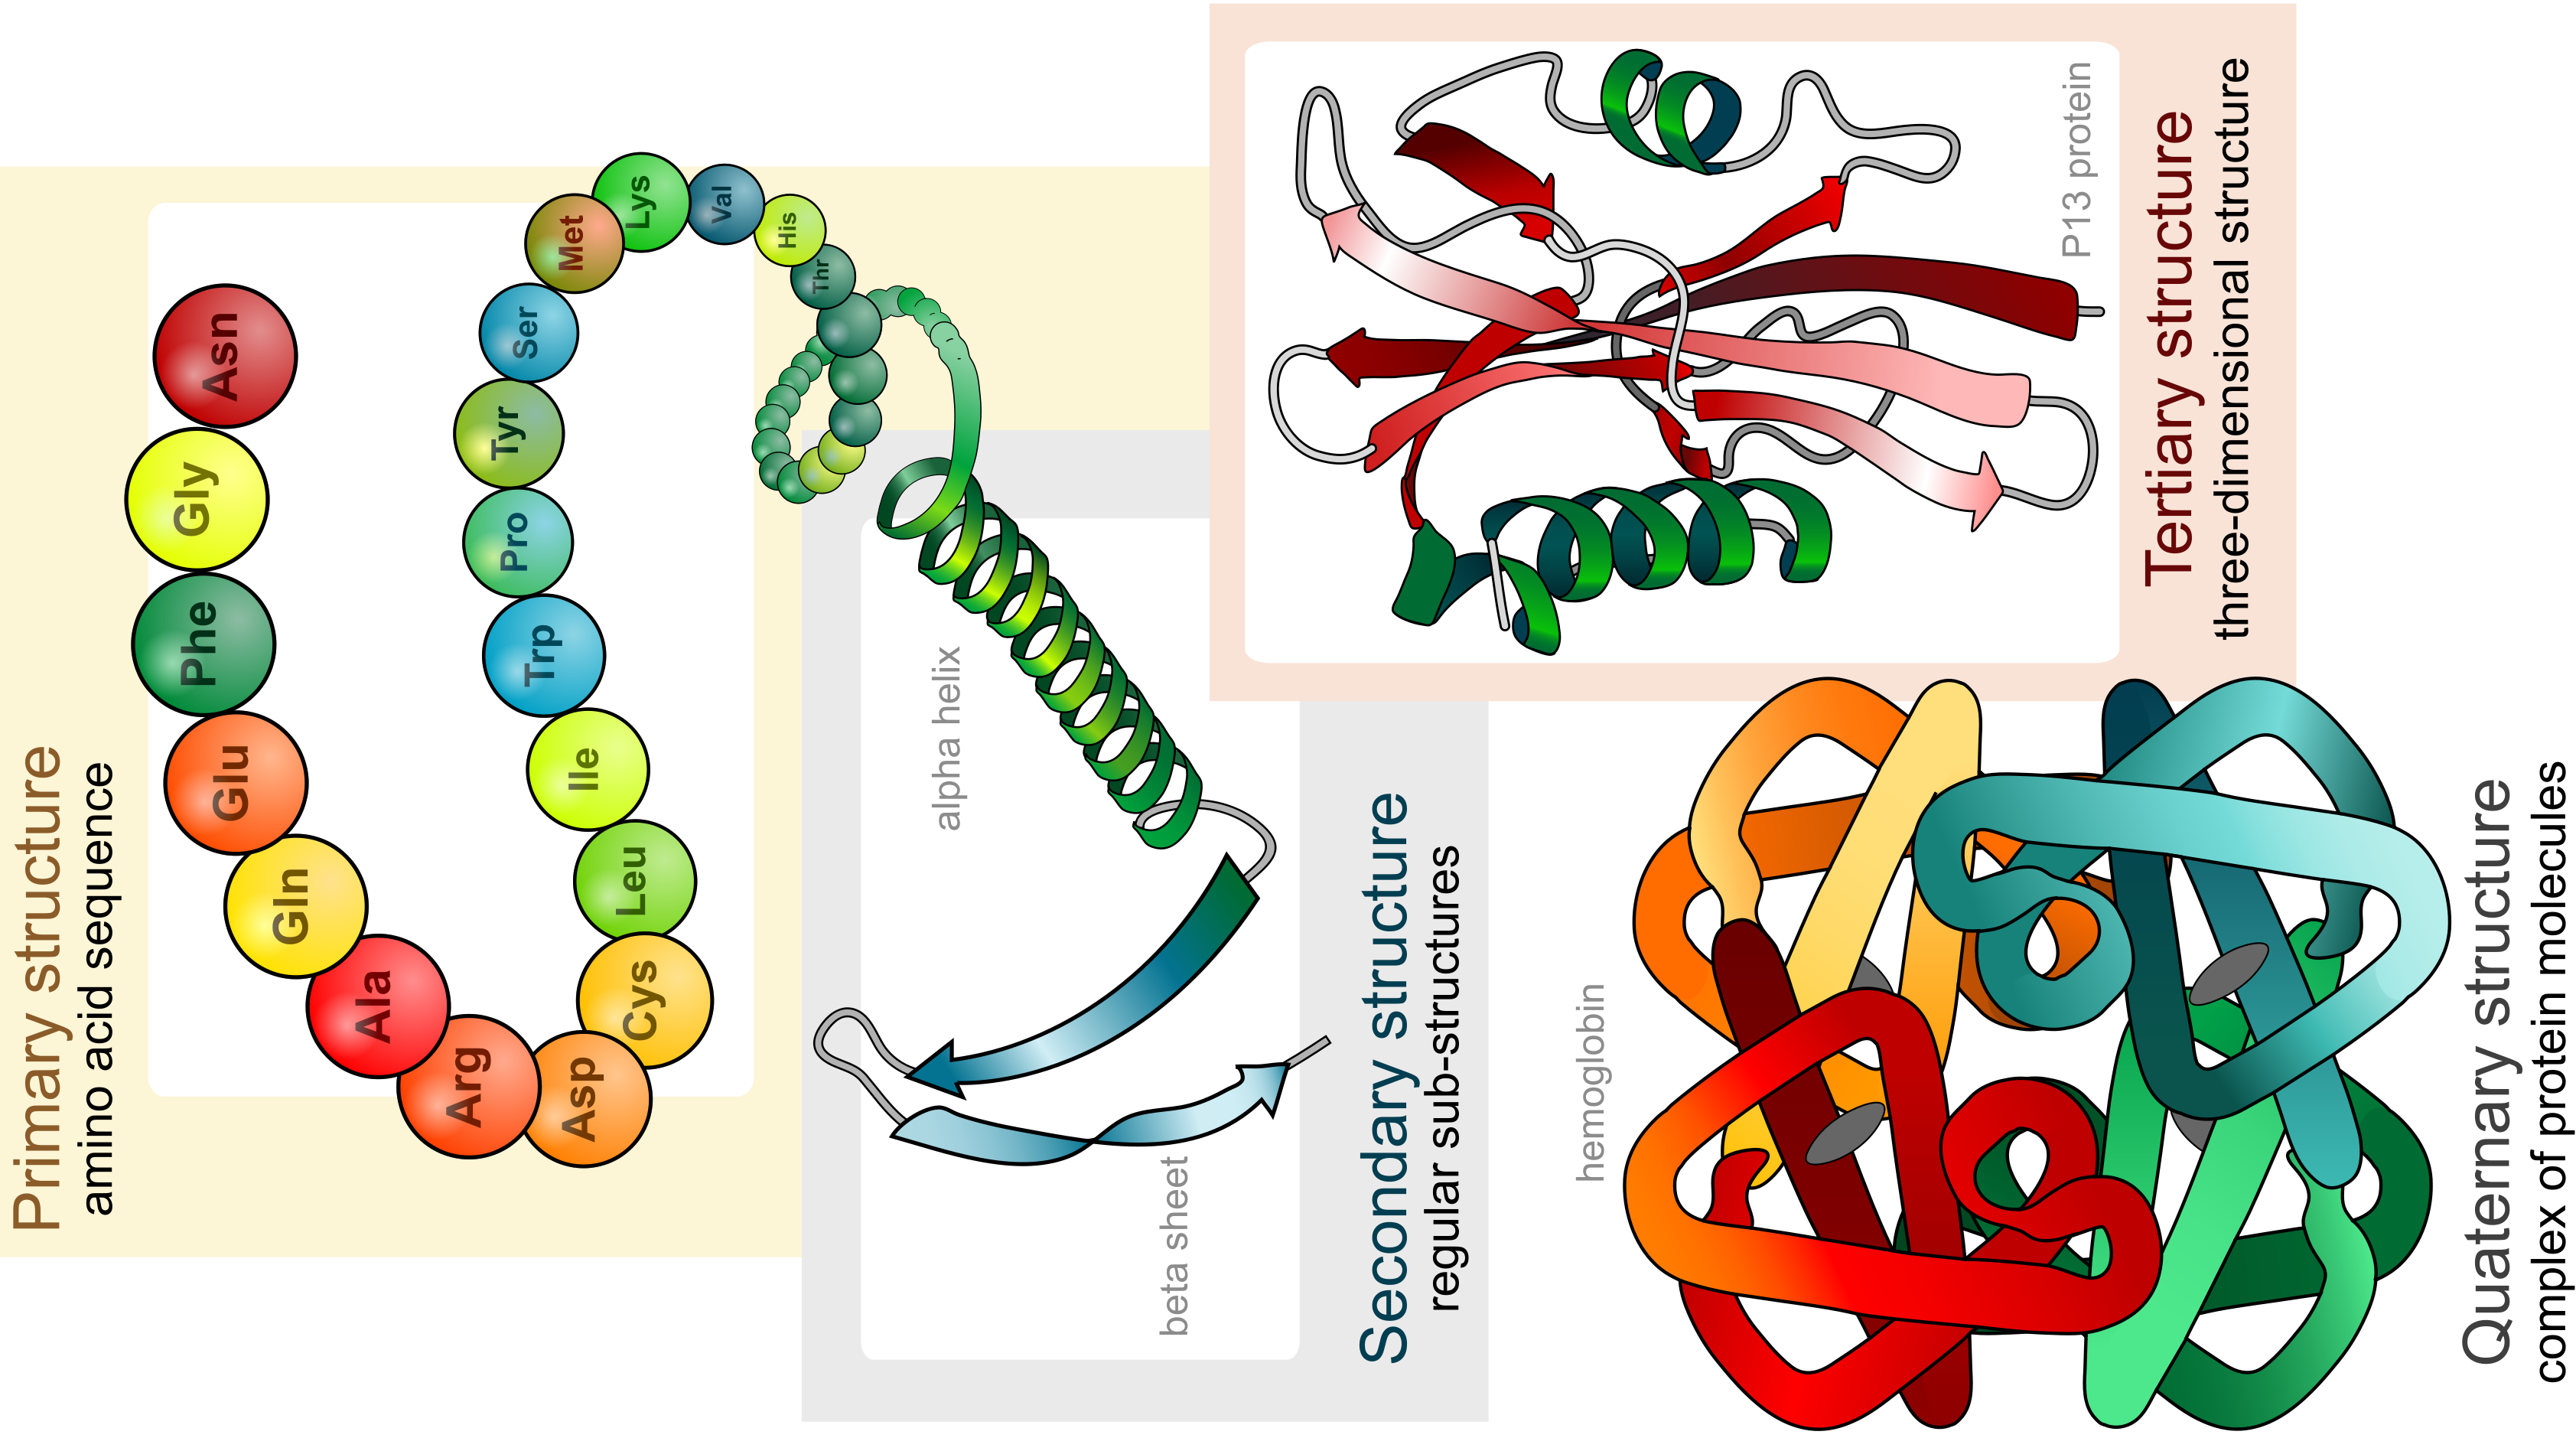
\includegraphics[width=11.5cm]{c1.intro.protein.01.png}
  \end{figure}
\end{frame}

\begin{frame}
  \frametitle{生物学 | \alert{数据库}}
  \begin{figure}
    \centering
    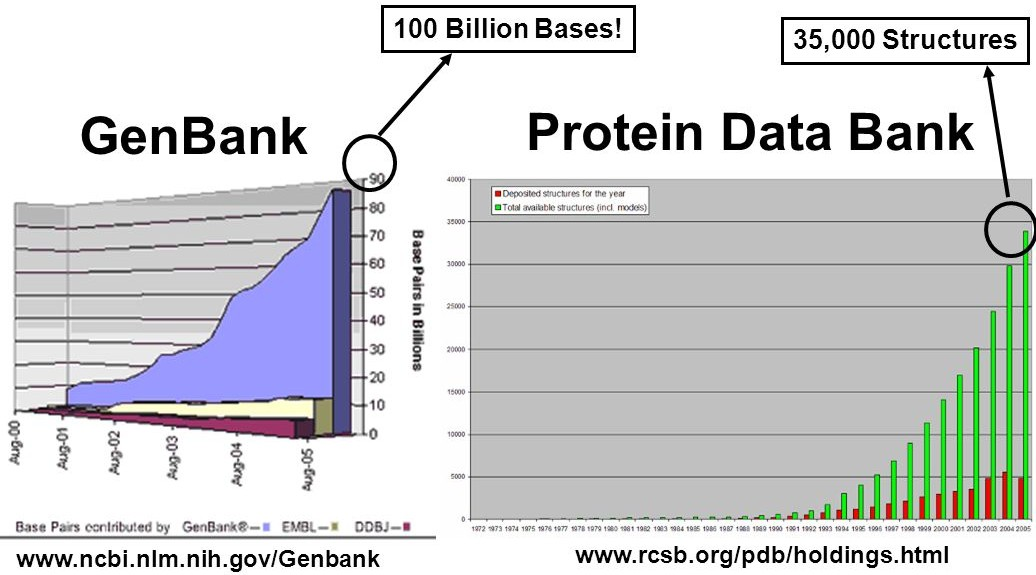
\includegraphics[width=11cm]{c1.intro.db.01.jpg}
  \end{figure}
\end{frame}

\begin{frame}
  \frametitle{生物学 | 数据格式}
  \begin{figure}
    \centering
    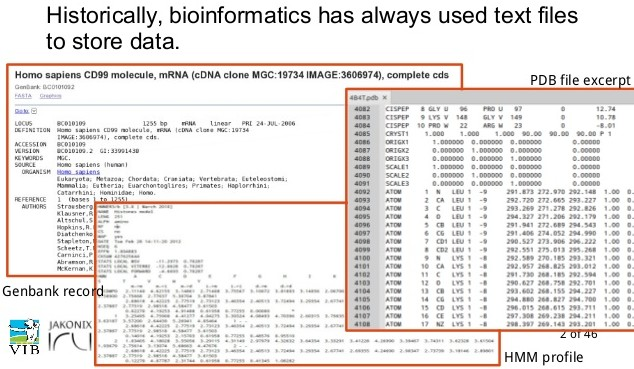
\includegraphics[width=11cm]{c1.intro.data.format.01.jpg}
  \end{figure}
\end{frame}

\section{计算机科学}
\begin{frame}
  \frametitle{计算机科学 | 历史}
  \begin{figure}
    \centering
    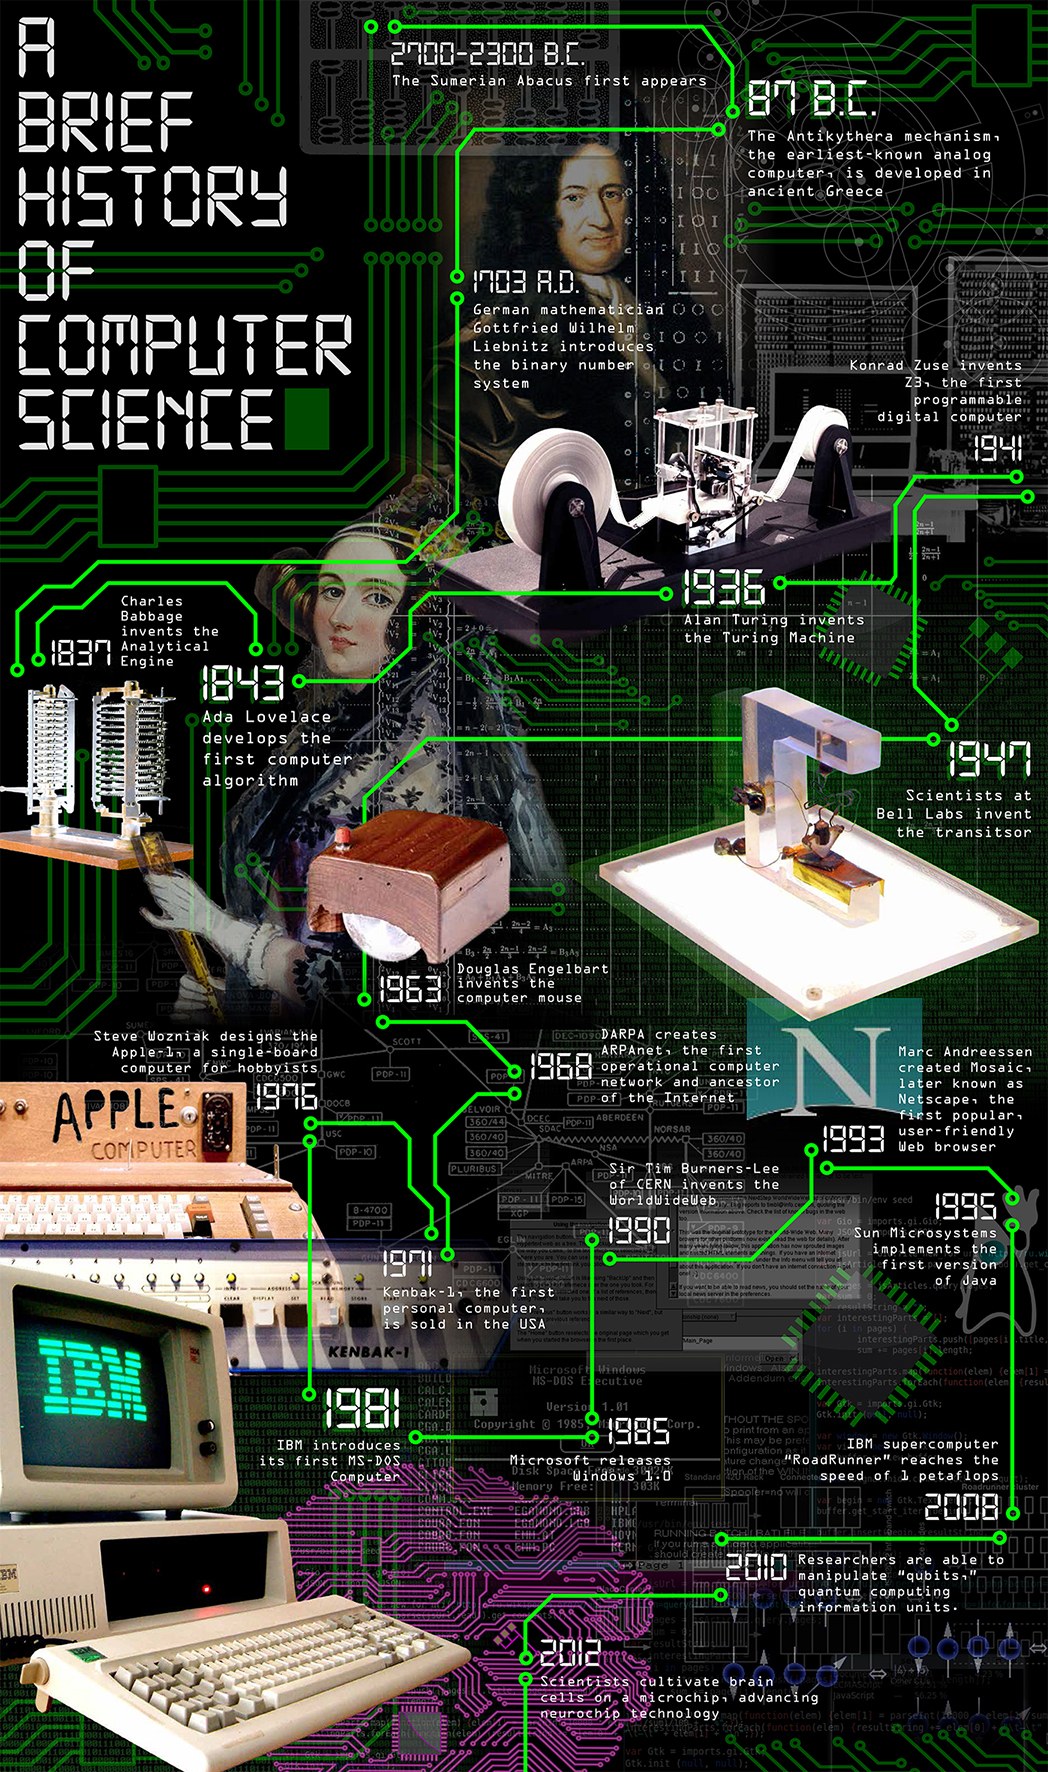
\includegraphics[width=10cm,height=7.5cm]{c1.intro.cs.history.01.png}
  \end{figure}
\end{frame}

\begin{frame}
  \frametitle{计算机科学 | \alert{术语}}
  \begin{block}{\textit{in vivo}}
  \textit{In vivo}为拉丁文“在活体内”之意。在科学文献中,\textit{in vivo}常指进行于完整且存活的个体内的组织的实验,以区别在生物体上移除下来的组织或死亡的组织上进行的实验(对应的拉丁文为\textit{in vitro })。
  \end{block}
  \pause
  \begin{block}{\textit{in vitro}}
    \textit{In vitro}是拉丁语中“在玻璃里”的意思,意指进行或发生于试管内的实验与实验技术。更广义的意思,则指活生物体之外的环境中的操作。
  \end{block}
  \pause
  \begin{block}{\textit{in silico}}
    \textit{In
    silico}是指“在硅之中”,也就是说“进行于电脑中,或是经由电脑模拟”之意,此用语是衍生自另外两个在生物学上常用的短语:\textit{in vivo}(生物活体内)及\textit{in vitro}(生物活体外)。
  \end{block}
\end{frame}

\begin{frame}
  \frametitle{计算机科学 | 编程语言}
  \begin{figure}
    \centering
    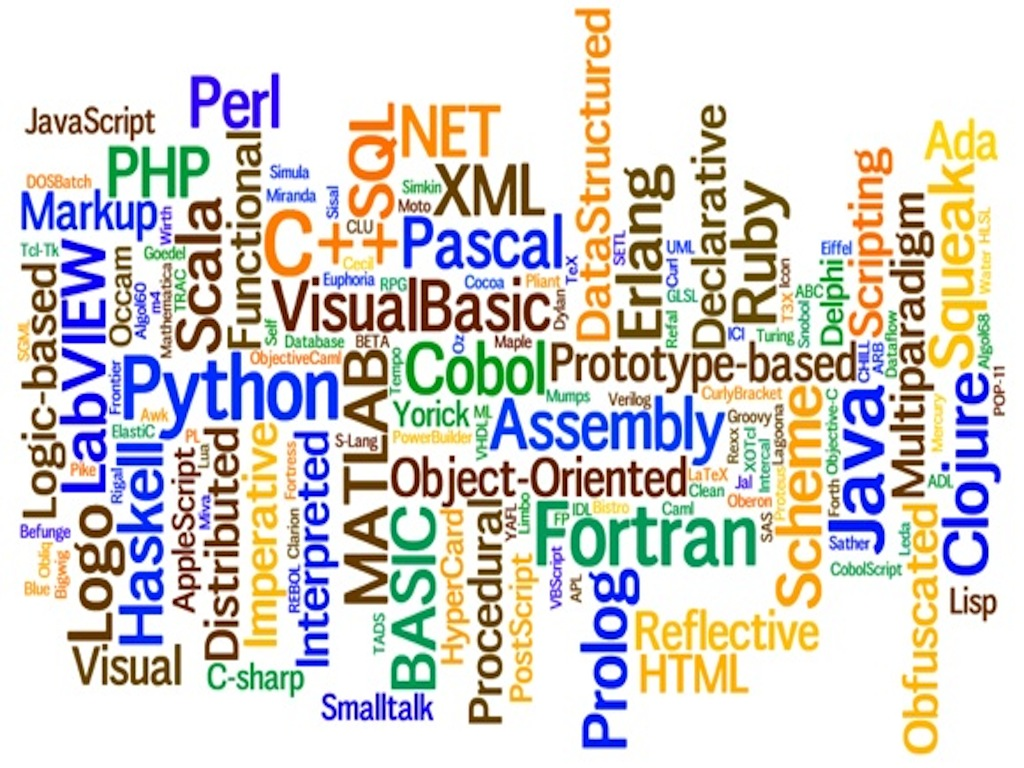
\includegraphics[width=10cm]{c1.intro.language.jpg}
  \end{figure}
\end{frame}

\begin{frame}
  \frametitle{计算机科学 | 编程语言 | 崇拜/鄙视链}
  \begin{figure}
    \centering
    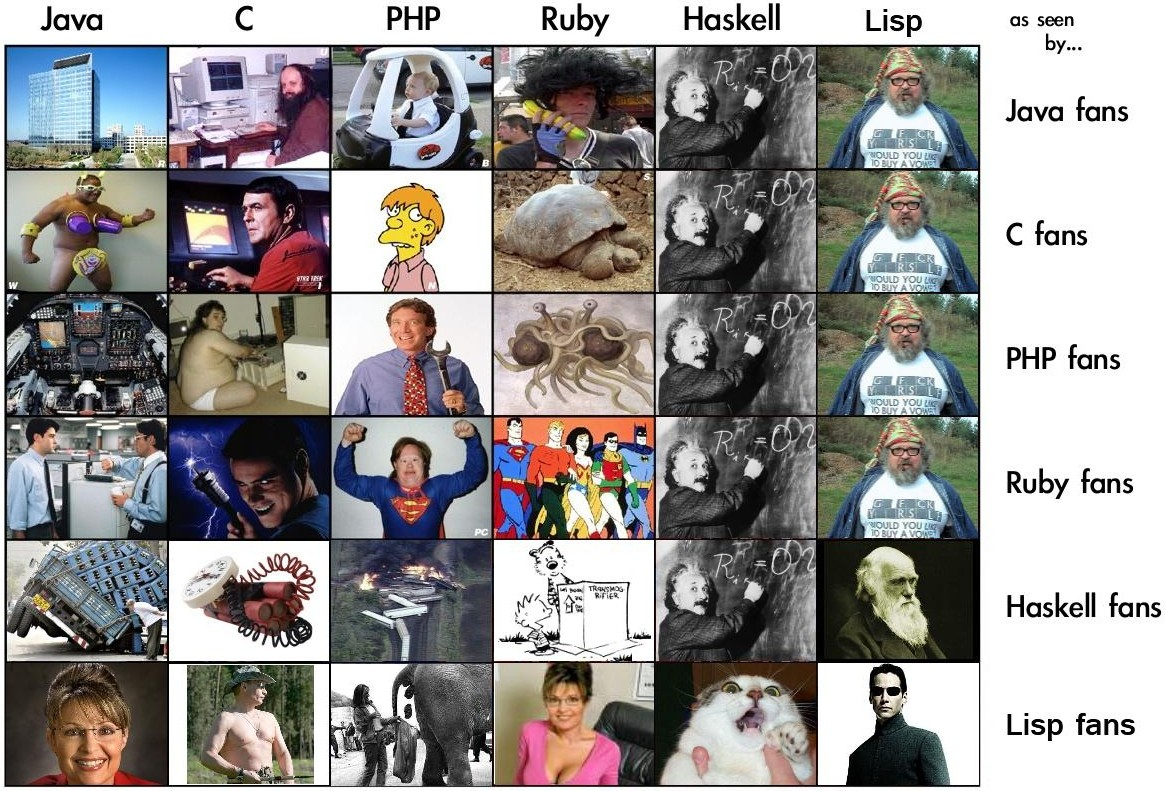
\includegraphics[width=11cm]{c1.intro.language.fanboys.jpg}
  \end{figure}
\end{frame}

\begin{frame}
  \frametitle{计算机科学 | 编程语言 | 特色}
  \begin{figure}
    \centering
    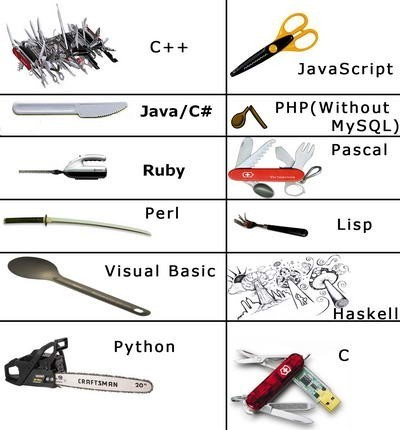
\includegraphics[width=7cm]{c1.intro.language.knife.jpg}
  \end{figure}
\end{frame}

\begin{frame}
  \frametitle{计算机科学 | 编程语言 | 流行度}
  \begin{figure}
    \centering
    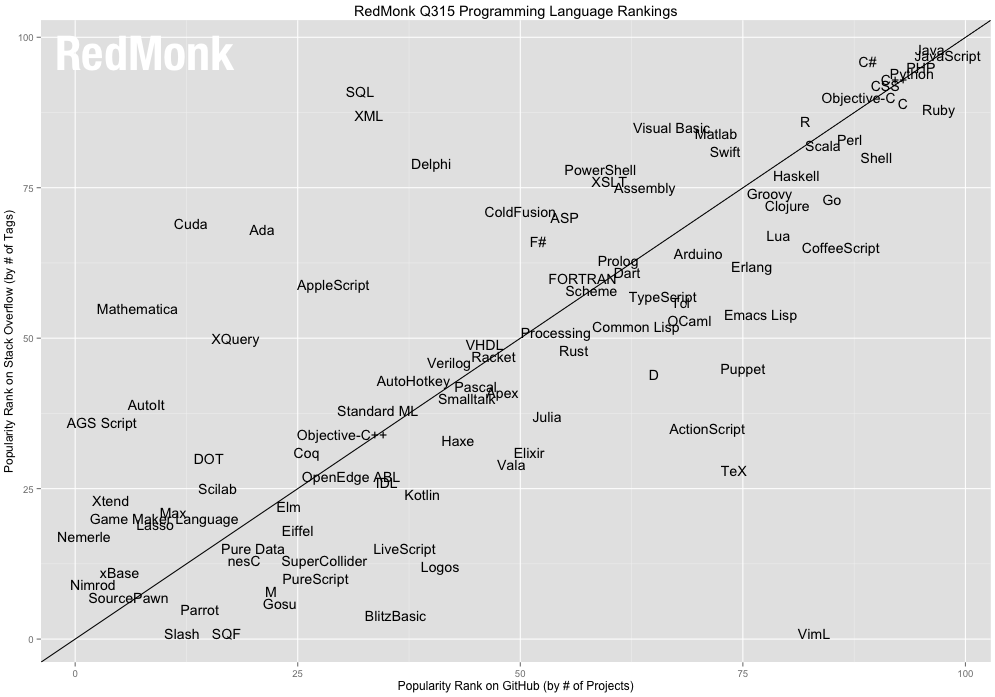
\includegraphics[width=11cm]{c1.intro.language.rank.png}
  \end{figure}
\end{frame}

\begin{frame}
  \frametitle{计算机科学 | 编程语言 | 排名}
  \begin{figure}
    \centering
    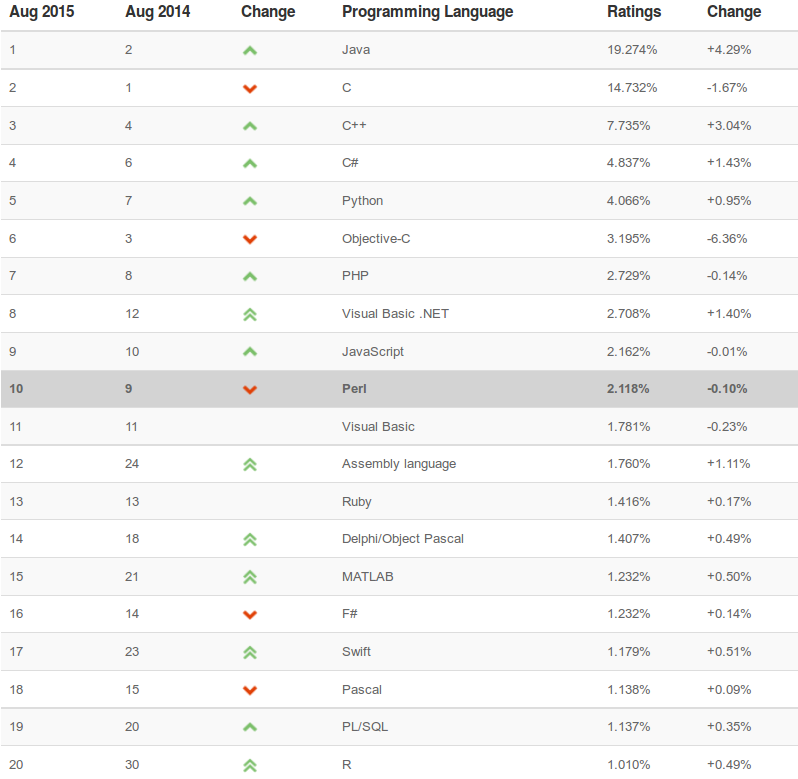
\includegraphics[width=10cm]{c1.intro.language.rate.png}
  \end{figure}
\end{frame}

\begin{frame}
  \frametitle{计算机科学 | 编程语言 | 生物信息学}
  \begin{block}{\alert{生物信息学常用编程语言}}
    Perl(1987)、Python(1991)、Ruby(1995)、Java(1995)
  \end{block}
  \begin{figure}
    \centering
    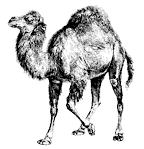
\includegraphics[width=2.5cm]{c1.intro.perl.logo.png}
    \hspace{2em}
    
\includegraphics[width=5.5cm]{c1.intro.python.logo.png}\\
    
\includegraphics[width=2cm]{c1.intro.ruby.logo.png}
    \hspace{11em}
    
\includegraphics[width=1.5cm]{c1.intro.java.logo.png}
  \end{figure}
\end{frame}

\begin{frame}
  \frametitle{计算机科学 | 编程语言 | BioX}
  \begin{block}{\alert{生物信息学专用}}
    BioPerl、Biopython、BioRuby、BioJava
  \end{block}
  \begin{figure}
    \centering
    
\includegraphics[width=2.5cm]{c1.intro.bioperl.logo.png}
    \hspace{2em}
    
\includegraphics[width=6cm]{c1.intro.biopython.logo.jpg}\\
    
\includegraphics[width=2cm]{c1.intro.bioruby.logo.png}
    \hspace{10em}
    
\includegraphics[width=3cm]{c1.intro.biojava.logo.jpg}
  \end{figure}
\end{frame}

\section{编程}
\begin{frame}
  \frametitle{编程 | 与生物信息学}
  \begin{block}{不需要!}
    \begin{itemize}
      \item 有现成的工具可以使用
      \item 五湖四海皆兄弟
      \item 有钱能使磨推鬼
      \item ……
    \end{itemize}
  \end{block}
  \pause
  \begin{block}{需要!}
    \begin{itemize}
      \item 没有现成的工具
      \item 兄弟们都在忙着混江湖
      \item 工资涨如龟速,物价涨如赤兔
      \item ……
    \end{itemize}
  \end{block}
\end{frame}

\begin{frame}
  \frametitle{编程 | 值得学习}
  \begin{itemize}
    \item 有助于理解现有工具的配置与个性化修改
    \item 编写程序来批量运行现有程序
    \item
      数据分析很简单,前期数据处理很难难难……(二八定律,80/20法则,帕雷托法则)
    \item 增强研究工作的可重复性
    \item 人生苦短,学习编程
    \item ……
  \end{itemize}
\end{frame}

\begin{frame}
  \frametitle{编程 | 与艺术}
  \begin{figure}
    \centering
    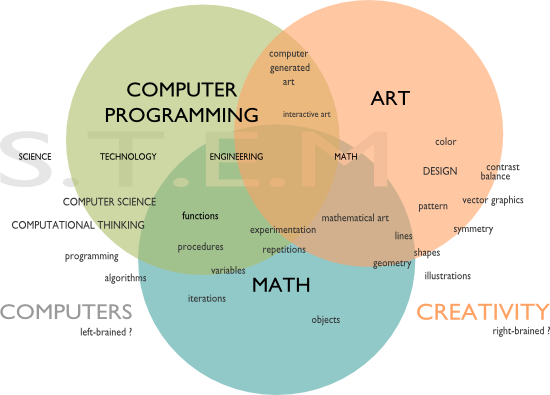
\includegraphics[width=10cm]{c1.intro.programming.art.01.png}
  \end{figure}
\end{frame}

\begin{frame}
  \frametitle{编程 | 与艺术}
  \begin{center}
    \large{每一位程序员都是一位艺术家!\\
    每一个程序都是一件艺术品!\\
    编写程序 = 艺术创作!}
\end{center}
\vspace{-1em}
  \begin{figure}
    \centering
    
\includegraphics[width=10.5cm]{c1.intro.programming.art.02.jpg}
  \end{figure}
\end{frame}

\begin{frame}
  \frametitle{编程 | 局限 | 理论上无解}
  \begin{block}{任务}
    \begin{enumerate}
      \item<1-> 同时精确测量粒子的位置和动量
      \item<2-> 寻找第四种可以镶嵌平面的凸六边形
      \item<3-> 寻找可以镶嵌平面的边数大于6的凸多边形
      \item<4-> 分析敲除所有必需基因后的基因表达
    \end{enumerate}
  \end{block}
  \begin{block}{原理}
    \begin{enumerate}
      \item<1-> 海森堡不确定性原理
      \item<2-> 有且只有三种凸六边形可以镶嵌平面
      \item<3-> 边数大于6的凸多边形都无法镶嵌平面
      \item<4-> 都说了是必需基因……
    \end{enumerate}
  \end{block}
\end{frame}

\begin{frame}
  \frametitle{编程 | 局限 | 实际上不可解}
  \begin{block}{任务}
    \begin{enumerate}
      \item<1-> 破解RSA秘钥
      \item<2-> 暴力破解由94个字符(26小写、26大写、10数字、32标点)随机组合成的长12个字符的密码
      \item<3-> 蛋白质折叠中通过随机尝试找到总能量最低的构象状态
    \end{enumerate}
  \end{block}
  \begin{block}{原因}
    \begin{enumerate}
      \item<1-> 对极大整数做因数分解非常困难(破解RSA-2048(2048-bit)的密钥可能需要耗费传统电脑10亿年的时间,而量子计算机只需要100秒就可以完成。)【量子计算机+秀尔算法】
      \item<2-> 普通台式机,每秒运算40亿次,需要大约30万年以上才能破解
      \item<3-> 利文索尔佯谬(Levinthal's paradox):100氨基酸,每个2种构象,每次尝试耗时$10^{-13}$s,穷举需要40亿年
    \end{enumerate}
  \end{block}
\end{frame}

\section{Bioinformatics Career Survey 2008}
\begin{frame}
  \frametitle{2008 | happiness}
   \begin{figure}
     \centering
     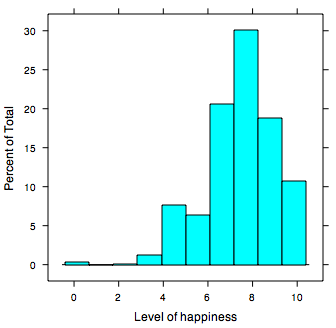
\includegraphics[width=0.65\textwidth]{c1.intro.2008.happiness.png}
   \end{figure} 
\end{frame}

\begin{frame}
  \frametitle{2008 | happiness vs. career position}
   \begin{figure}
     \centering
     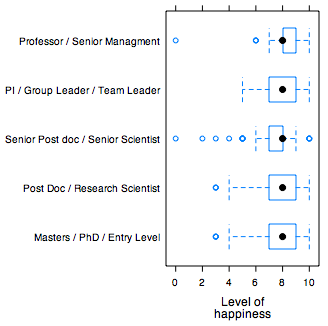
\includegraphics[width=0.65\textwidth]{c1.intro.2008.happiness.position.png}
   \end{figure} 
\end{frame}

\begin{frame}
  \frametitle{2008 | likes vs. dislikes}
   \begin{figure}
     \centering
     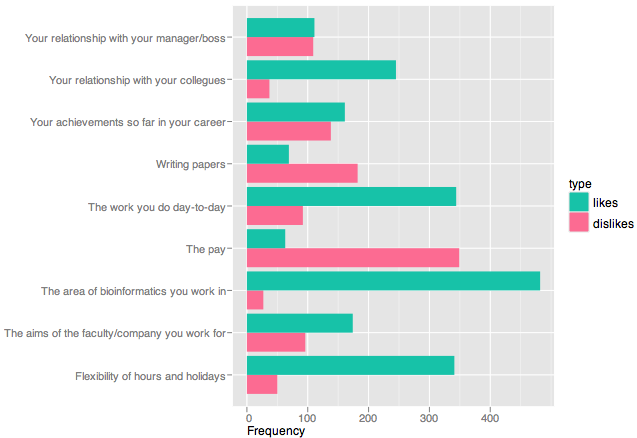
\includegraphics[width=0.9\textwidth]{c1.intro.2008.happiness.like.png}
   \end{figure} 
\end{frame}

\begin{frame}
  \frametitle{2008 | research area}
   \begin{figure}
     \centering
     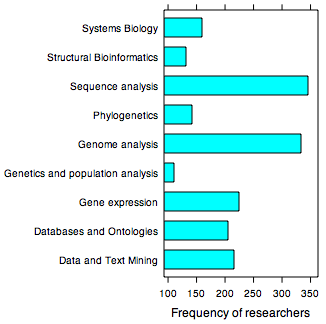
\includegraphics[width=0.65\textwidth]{c1.intro.2008.area.png}
   \end{figure} 
\end{frame}

\begin{frame}
  \frametitle{2008 | research area | clustering}
   \begin{figure}
     \centering
     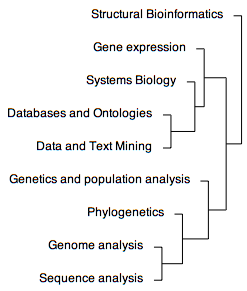
\includegraphics[width=0.55\textwidth]{c1.intro.2008.area.cluster.png}
   \end{figure} 
\end{frame}

\begin{frame}
  \frametitle{2008 | background}
   \begin{figure}
     \centering
     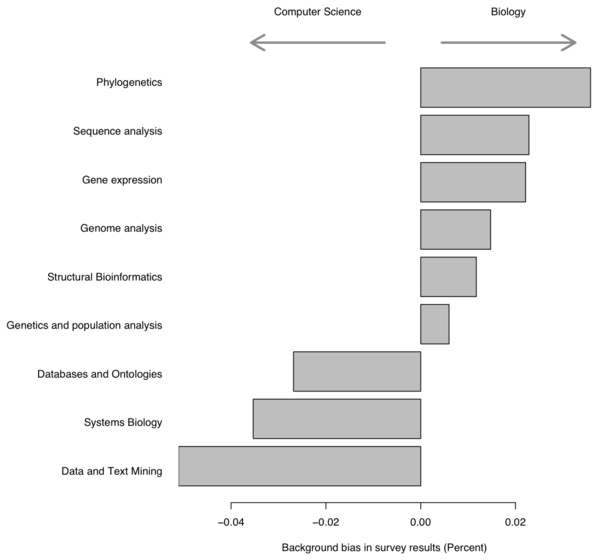
\includegraphics[width=0.7\textwidth]{c1.intro.2008.background.png}
   \end{figure} 
\end{frame}

\begin{frame}
  \frametitle{2008 | language}
   \begin{figure}
     \centering
     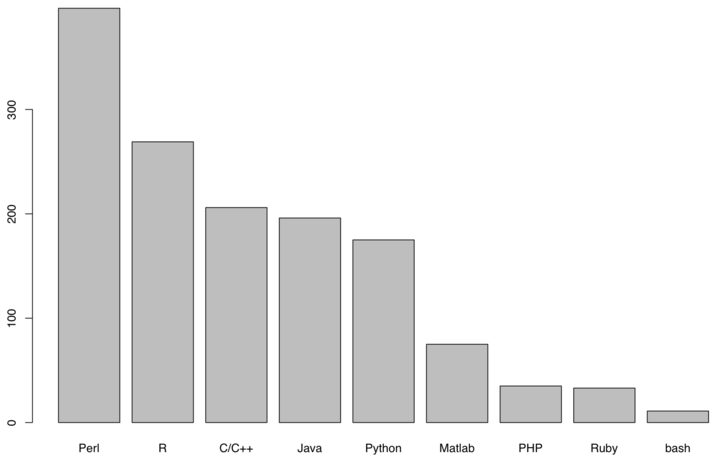
\includegraphics[width=0.9\textwidth]{c1.intro.2008.language.png}
   \end{figure} 
\end{frame}

\begin{frame}
  \frametitle{2012 | language}
   \begin{figure}
     \centering
     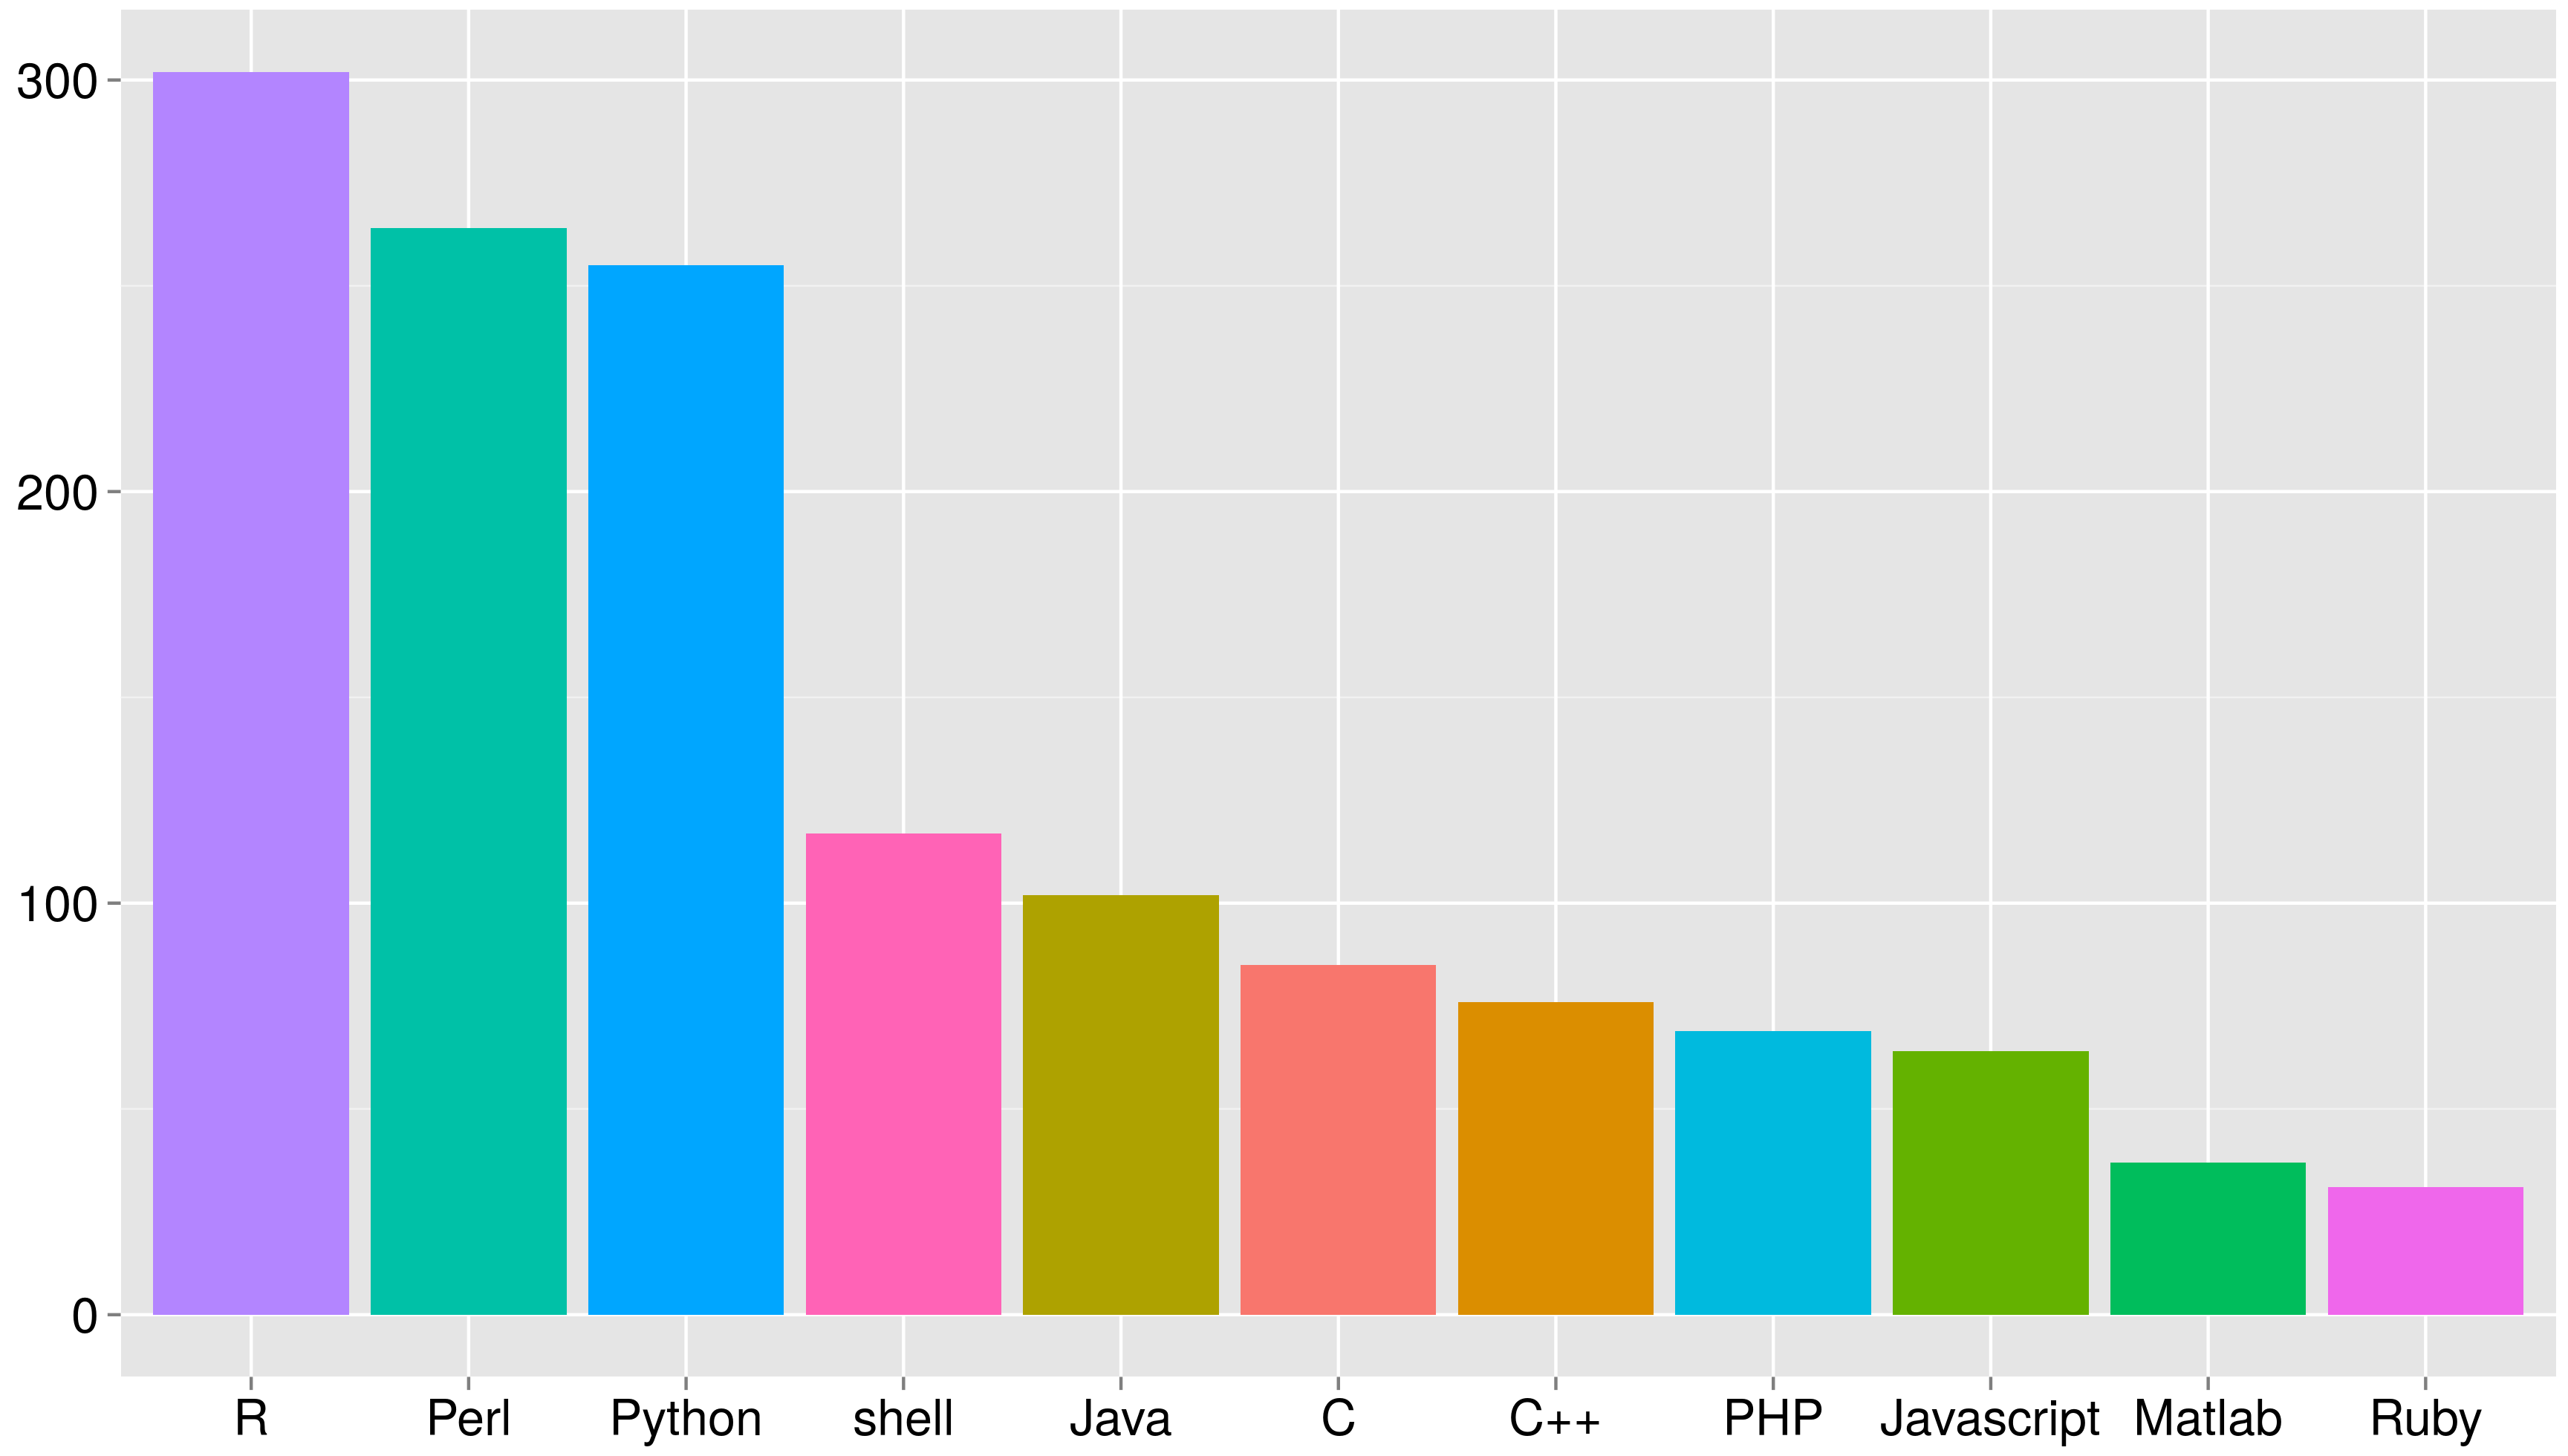
\includegraphics[width=0.95\textwidth]{c1.intro.2012.language.png}
   \end{figure} 
\end{frame}

\begin{frame}
  \frametitle{2008 | applications}
   \begin{figure}
     \centering
     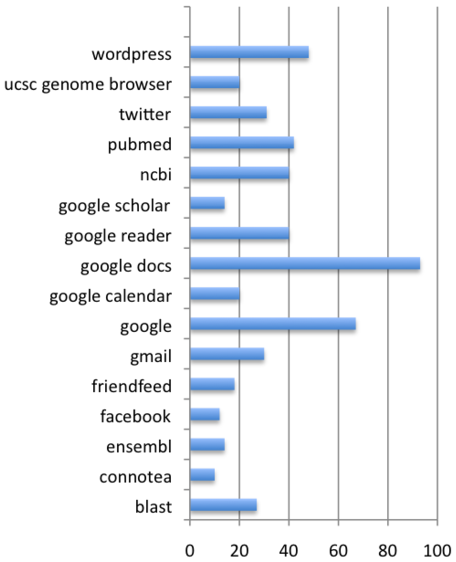
\includegraphics[width=0.53\textwidth]{c1.intro.2008.application.png}
   \end{figure} 
\end{frame}

\begin{frame}
  \frametitle{2008 | tools}
   \begin{figure}
     \centering
     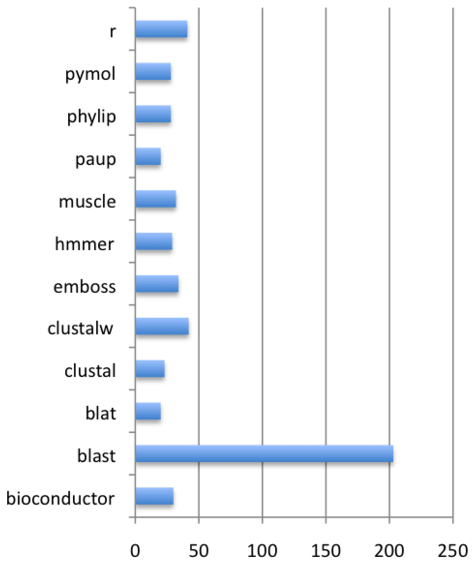
\includegraphics[width=0.55\textwidth]{c1.intro.2008.tool.png}
   \end{figure} 
\end{frame}

\begin{frame}
  \frametitle{2008 | salary}
  \begin{block}{industry vs. academic}
    \begin{itemize}
      \item Academic Salary Mean/Median: \$36,520 / \$33,712
      \item Industry Salary Mean/Median: \$66,239 / \$64,235 
    \end{itemize}
  \end{block}
  \pause
  \begin{block}{Salary/Years Experience}
    \begin{itemize}
      \item Academic Mean/Median: \$10,970 / \$8,333
      \item Industry Mean/Median: \$17,410 / \$12,000 
    \end{itemize}
  \end{block}
\end{frame}

\begin{frame}
  \frametitle{2008 | 参考资料}
  \begin{itemize}
    \item \href{http://openwetware.org/wiki/Biogang:Projects/Bioinformatics\_Career\_Survey\_2008}{Bioinformatics Career Survey 2008}
    \item \href{http://openwetware.org/wiki/Biogang:Projects/Bioinformatics\_Career\_Survey\_2008\_Results}{Bioinformatics Career Survey 2008 Results}
    \item \href{https://github.com/michaelbarton/bioinformatics-career-survey}{bioinformatics-career-survey (GitHub)}
    \item \href{http://www.ncbi.nlm.nih.gov/pmc/articles/PMC2267699/}{A comparison of common programming languages used in bioinformatics} 
    \item \href{http://www.molecularecologist.com/2012/11/a-comparison-of-bioinformatics-programming-languages/}{A comparison of bioinformatics programming languages} 
    \item \href{https://nlcb.wordpress.com/2013/02/23/programming-languages-of-bioinformatics-2/}{Programming Languages of Bioinformatics} 
  \end{itemize}
\end{frame}

\section{回顾与总结}
\subsection{总结}
\begin{frame}
  \frametitle{绪论 | 总结}
  \begin{block}{知识点}
    \begin{itemize}
      \item 生物信息学:交叉学科,多种技能,领域宽泛
      \item 生物学:DNA,RNA,蛋白质
      \item 计算机科学:三个术语,编程语言
    \end{itemize}
  \end{block}
\end{frame}

\subsection{思考题}
\begin{frame}
  \frametitle{绪论 | 思考题}
  \begin{enumerate}
    \item 生物信息学主要是由哪些学科交叉而来的?
    \item 生物信息学主要需要哪些方面的知识和技能?
    \item DNA是由哪四种碱基组成的?RNA与之有何不同?
    \item 列举常见的20种氨基酸,它们三字母和单字母的缩写分别是什么?
    \item 列举常见的存储DNA序列和蛋白质结构的数据库。
    \item \textit{in vivo}、\textit{in vitro}和\textit{in silico}分别代表什么含义?
    \item 列举常见的编程语言,在生物信息学中常用的编程语言,专用于生物信息学的工具集。
  \end{enumerate}
\end{frame}

\begin{frame}
  \frametitle{下节预告}
  \begin{block}{Markdown}
    回顾、总结Markdown标记语言的基本语法:
    \begin{itemize}
      \item 标题
      \item 强调
      \item 列表
      \item 代码
      \item 引用
      \item 链接
      \item ……
    \end{itemize}
  \end{block}
\end{frame}


\section*{Acknowledgements}
\begin{frame}
  \frametitle{Powered by}
  \begin{center}
    
\includegraphics[width=9cm]{power.png}
  \end{center}
\end{frame}

\end{document}

